% This document should be compiled with XeLaTeX. 
\documentclass[preprint,11pt,authoryear,3p]{elsarticle}

%% Use the option review to obtain double line spacing
%% \documentclass[preprint,review,12pt]{elsarticle}

%% Use the options 1p,twocolumn; 3p; 3p,twocolumn; 5p; or 5p,twocolumn
%% for a journal layout:
%% \documentclass[final,1p,times]{elsarticle}
%% \documentclass[final,1p,times,twocolumn]{elsarticle}
%% \documentclass[final,3p,times]{elsarticle}
%% \documentclass[final,3p,times,twocolumn]{elsarticle}
%% \documentclass[final,5p,times]{elsarticle}
%% \documentclass[final,5p,times,twocolumn]{elsarticle}

%% For including figures, graphicx.sty has been loaded in
%% elsarticle.cls. If you prefer to use the old commands
%% please give \usepackage{epsfig}
\usepackage{subfigure}

%% The amssymb package provides various useful mathematical symbols
\usepackage{amssymb}
%% The amsthm package provides extended theorem environments
% \usepackage{amsthm}
\usepackage{amsmath}

%% The lineno packages adds line numbers. Start line numbering with
%% \begin{linenumbers}, end it with \end{linenumbers}. Or switch it on
%% for the whole article with \linenumbers.
\usepackage{lineno}
\usepackage{lscape}
%% Set the font style of the main text as the times new roman
% \usepackage{fontspec}
% \setmainfont{Times New Roman}
% \renewcommand{\familydefault}{\rmdefault}

%% Add the command "\autoref{}"
\usepackage{hyperref}
%% Add the command "\hl{}"
\usepackage{soul, color, xcolor}
\usepackage{threeparttable}
\usepackage{longtable}
\usepackage{array}
\usepackage{setspace}
\usepackage{tabularx}
\usepackage{array}
\usepackage{amsmath} % 推荐,用于数学公式
\usepackage{algorithm}
\usepackage{algpseudocode} % 使用这个宏包
\usepackage{pifont}
\newcommand{\cmark}{\(\checkmark\)} % 对勾
\newcommand{\tmark}{\(\triangle\)}   % 空心三角
\newcommand{\nmark}{\(-\)}           % 横杠
\newcommand{\xmark}{$\times$}          % 不推荐

\usepackage{geometry}
\geometry{left=2cm, right=2cm, top=2cm, bottom=2cm}

\biboptions{sort&compress}%参考文献可以压缩显示例如1-3

% \renewcommand{\figurename}{\bf{Fig.}} %修改标题样式
\renewcommand{\figureautorefname}{Fig.}
\renewcommand{\tablename}{\bf{Table}}
\renewcommand{\equationautorefname}{Eq.}
\renewcommand{\sectionautorefname}{Sec.}
\renewcommand{\subsectionautorefname}{Sec.}
\renewcommand{\subsubsectionautorefname}{Sec.}
\usepackage[skip=5pt]{caption}
\captionsetup[figure]{name={Fig.},labelsep=period}
\captionsetup[table]{name={Table},labelsep=period}
\captionsetup{labelfont=bf}

% --- 将以下代码放入导言区 ---
\setlength{\textfloatsep}{10pt plus 1.0pt minus 2.0pt}
\setlength{\floatsep}{8pt plus 1.0pt minus 2.0pt}
\setlength{\intextsep}{8pt plus 1.0pt minus 2.0pt}
\setlength{\abovecaptionskip}{3pt plus 2pt minus 2pt}
\setlength{\belowcaptionskip}{3pt plus 2pt minus 2pt}

\usepackage{booktabs}
\usepackage{multirow}

%% Set the space between two lines of text next to each other.
\usepackage{setspace}
\renewcommand{\baselinestretch}{1.5}
% \setlength{\baselineskip}{24pt}


% \journal{Automation in Construction}

\begin{document}
\linenumbers

% modify the line space between the text and equation.
\setlength{\abovedisplayskip}{-15pt}
% \setlength{\abovedisplayshortskip}{0pt}
\setlength{\belowdisplayskip}{-0pt}
% \setlength{\belowdisplayshortskip}{-12pt}

\begin{frontmatter}

%% Title, authors and addresses

%% use the tnoteref command within \title for footnotes;
%% use the tnotetext command for theassociated footnote;
%% use the fnref command within \author or \address for footnotes;
%% use the fntext command for theassociated footnote;
%% use the corref command within \author for corresponding author footnotes;
%% use the cortext command for theassociated footnote;
%% use the ead command for the email address,
%% and the form \ead[url] for the home page:
%% \title{Title\tnoteref{label1}}
%% \tnotetext[label1]{}
%% \author{Name\corref{cor1}\fnref{label2}}
%% \ead{email address}
%% \ead[url]{home page}
%% \fntext[label2]{}
%% \cortext[cor1]{}
%% \affiliation{organization={},
%%             addressline={},
%%             city={},
%%             postcode={},
%%             state={},
%%             country={}}
%% \fntext[label3]{}

\title{A State-of-the-Art Review on the Space-Air-Ground Integrated Intelligent Monitoring for Large-scale Deep Excavation Engineering}

%% use optional labels to link authors explicitly to addresses:
%% \author[label1,label2]{}
%% \affiliation[label1]{organization={},
%%             addressline={},
%%             city={},
%%             postcode={},
%%             state={},
%%             country={}}
%%
%% \affiliation[label2]{organization={},
%%             addressline={},
%%             city={},
%%             postcode={},
%%             state={},
%%             country={}}

\author[Ori1]{Qiwei Wan\fnref{firstAu}}
\author[Ori1,Ori2]{Changjie Xu\corref{cor1}}
% \author[Ori3]{Xiangyu Wang}
\author[Ori1]{Kewang Zhang}
\author[Ori1]{Haibin Ding}
\author[Ori2]{Gang Wei}

\fntext[firstAu]{State Key Laboratory of Safety and Resilience of Civil Engineering in Mountain Area, East China Jiaotong University, Nanchang, 330013, Jiangxi, China. E-mail address: wqw@ecjtu.edu.cn}
\cortext[cor1]{School of Civil Engineering and Architecture, East China Jiaotong University, Nanchang 330021,China. \\ E-mail address: xucj@zju.edu.cn}

\address[Ori1]{State Key Laboratory of Safety and Resilience of Civil Engineering in Mountain Area, East China Jiaotong University, Nanchang, 330013, Jiangxi, China.}

\address[Ori2]{College of Civil Engineering and Architecture, Zhejiang University, Hangzhou 310058, Zhejiang, China}

% \address[Ori3]{Australasian Joint Research Centre for Building Information Modelling, Curtin University,%Department and Organization
%             GPO Box U1987,
%             Nanchang,
%             WA 6845,
%             Perth,
%             Australia}


\begin{abstract}

Large urban foundation pits now generate sub-minute, multi-sensor data streams that challenge traditional ground-centric monitoring.  This study develops a Space-Air-Ground (SAG) framework that couples satellite InSAR, UAV photogrammetry/LiDAR and high-precision ground instruments to meet the dual targets of centimetre-level accuracy and 15-min decision latency required by modern observational codes.  A PRISMA-guided literature search (522 publications, 2010-2024) is distilled into three layers: (i) regulatory acceptance, (ii) data-fusion strategies and (iii) machine-learning toolkits.  First, a cross-regional code matrix reveals converging displacement limits $|Δu_{WT}|\le H/1000$ but divergent attitudes toward remote sensing, with Shanghai and Singapore mandating real-time SAG feeds, whereas UK and German standards remain optional.  Second, an applicability map links eight fusion algorithms to three operational scenarios—real-time filtering, post-hoc inversion and forecasting—showing that UKF/PF dominate sub-minute smoothing, D-S/Bayesian networks excel in asynchronous inversion, and hybrid CNN-LSTM or Transformer models achieve $\le$2.5 \% long-horizon MAPE.  Third, three mega-pit case studies (Shanghai East, Shenzhen CBD and Crossrail Farringdon) demonstrate that a tri-modal sensor portfolio can cut life-cycle monitoring cost by $\sim$40 \% while holding wall-top-displacement RMSE within ±2 mm.  The paper culminates in a seven-step implementation workflow—ranging from code-based threshold mapping to edge-cloud anomaly detection and AI-enhanced prognosis—and identifies sensor-physics limits, adaptive grid economics and physics-informed fusion as the key research frontiers.  The proposed framework converts SAG monitoring from a pilot-stage novelty into a reproducible, risk-responsive protocol for ever-deeper urban excavations.

\end{abstract}
%%Graphical abstract
% \begin{graphicalabstract}
% %\includegraphics{grabs}
% \end{graphicalabstract}

%%Research highlights
% \begin{highlights}
% \item Research highlight 1
% \item Research highlight 2
% \end{highlights}

\begin{keyword}
%% keywords here, in the form: keyword \sep keyword
% Multi-objective optimization \sep
% Enhanced genenic algorithm \sep
% Inverse design \sep
% Deformation control \sep
% Economic optimization 
%% PACS codes here, in the form: \PACS code \sep code

%% MSC codes here, in the form: \MSC code \sep code
%% or \MSC[2008] code \sep code (2000 is the default)

Space--Air--Ground monitoring \sep
Interferometric Synthetic Aperture Radar  \sep
Unmanned Aerial Vehicle photogrammetry \sep
Global Navigation Satellite System \sep
Multi-source data fusion \sep
Deep excavation
\end{keyword}

\end{frontmatter}

\section*{PRACTICAL APPLICATIONS}

The review turns a decade of scattered research into a turnkey playbook ready for specifications and bids: it first matches every key performance indicator—surface settlement, wall deflection, basal heave, strut force, pore pressure and vibration—to a “primary + redundant” sensor pair so that instrument accuracy is hard-wired to code triggers; recommends a tri-modal baseline of C/X-band InSAR, UAV LiDAR / photogrammetry and high-precision ground arrays that has already cut life-cycle monitoring costs by $\sim$40 \% while holding wall-top displacement within ± 2 mm on flagship mega-pits in Shanghai, Shenzhen and London; embeds a four-layer edge-to-cloud pipeline that keeps 95 \% of sensor updates inside the 15-minute observational-method window and supports automatic UAV or inclinometer re-tasks without new IT hardware; and provides a five-step rollout guide-threshold mapping, portfolio optimisation, latency budgeting, pilot calibration and full deployment-that operationalises SAG monitoring as a routine, code-compliant safeguard for ever-deeper urban excavations.

\section{Introduction}

Effective monitoring of large urban foundation pits is constrained by a persistent \emph{trilemma}: no single technology can simultaneously deliver city-scale \textbf{coverage}, millimetric \textbf{accuracy}, and minute-level \textbf{latency} required for risk-responsive construction control\citep{gong2019advances}. To break this impasse, we focus on deep excavations—typically exceeding 20 m and surrounded by vulnerable infrastructures—where conventional ground instrumentation alone is either too sparse or too slow to meet code-mandated deformation limits.  We argue that an integrated \emph{Space-Air-Ground} (SAG) framework, fusing satellite InSAR, UAV photogrammetry/LiDAR and in-situ sensor networks, offers a uniquely balanced solution: satellites provide synoptic settlement baselines, UAVs supply dense site models, and ground arrays capture causal subsurface responses.  Unlike previous reviews that discuss these tiers in isolation, this paper \textbf{distils} their complementary niches into a design-oriented roadmap tailored to excavation engineering.

\begin{figure}
    \centering
    \includegraphics[width=0.9\textwidth]{imgs/Multi_chars.pdf}
    \caption{Complex environment around the excavation project of Shanghai East Railway Station}
    \label{fig:complexEnvironment}
\end{figure}

Deep excavations—frequently exceeding 20 m and abutting sensitive infrastructure—intensify this conflict because conventional ground instruments alone are too sparse or too slow to satisfy code-mandated deformation limits \citep{AnIntegratedIntelligent}. An integrated SAG framework-combining satellite InSAR, UAV photogrammetry/LiDAR, and in-situ sensor networks—is therefore proposed as a balanced pathway: satellites supply synoptic settlement fields, UAVs deliver high-resolution site models, and ground arrays capture causal subsurface responses. Whereas earlier surveys consider these tiers in isolation, their complementarities are here \textbf{distilled} into a design-oriented roadmap tailored to excavation engineering.

The contributions of this study are threefold:  
(i) code requirements and sensor physics are synthesised into a KPI-sensor matrix that links each deformation index to its most suitable monitoring tier;  
(ii) published fusion strategies are critically reviewed, and their reported performance envelopes are mapped to typical excavation scenarios; and  
(iii) transferable lessons from representative SAG deployments are extracted to illustrate cost-benefit trade-offs and implementation pitfalls. Statistical evidence for the accelerating growth of SAG research is presented separately in \S\ref{sec:litsearch} to preserve concision.

The remainder of this paper is organised as follows: section 2 outlines the literature-search protocol; section 3 surveys monitoring technologies and governing standards; section 4 analyses multi-source fusion approaches; section 5 reviews engineering case studies; and section 6 discusses challenges, limitations, and future directions.

\section{Literature-Search Protocol and Bibliometric Results}

This chapter documents the systematic approach adopted to identify, screen, and profile state-of-the-art research on SAG monitoring for deep and large excavations. The workflow complies with the "Preferred Reporting Items for Systematic Reviews and Meta - Analyses extension for Scoping Reviews" (PRISMA-ScR) checklist for scoping reviews \citep{PRISMA-ScR}, with the process shown in \autoref{fig:ScreenProcess}.
Considering that SAG integrated monitoring technologies are applicable far beyond excavations, the scope of the literature search was expanded to the broader field of geotechnical engineering. When defining search queries in the Web of Science (WoS) database, both the characteristic technologies of SAG monitoring and the common monitoring objectives were taken into account. The final query adopted was: 

\begin{quote}
\texttt{TS=("deep excavation" OR "foundation pit" OR Geotechnical) AND
TS=("InSAR" OR "satellite radar" OR UAV OR "drone photogrammetry" OR LiDAR) AND
TS=("monitoring" OR deformation OR safety)}
\end{quote}

\begin{figure}
  \centering
  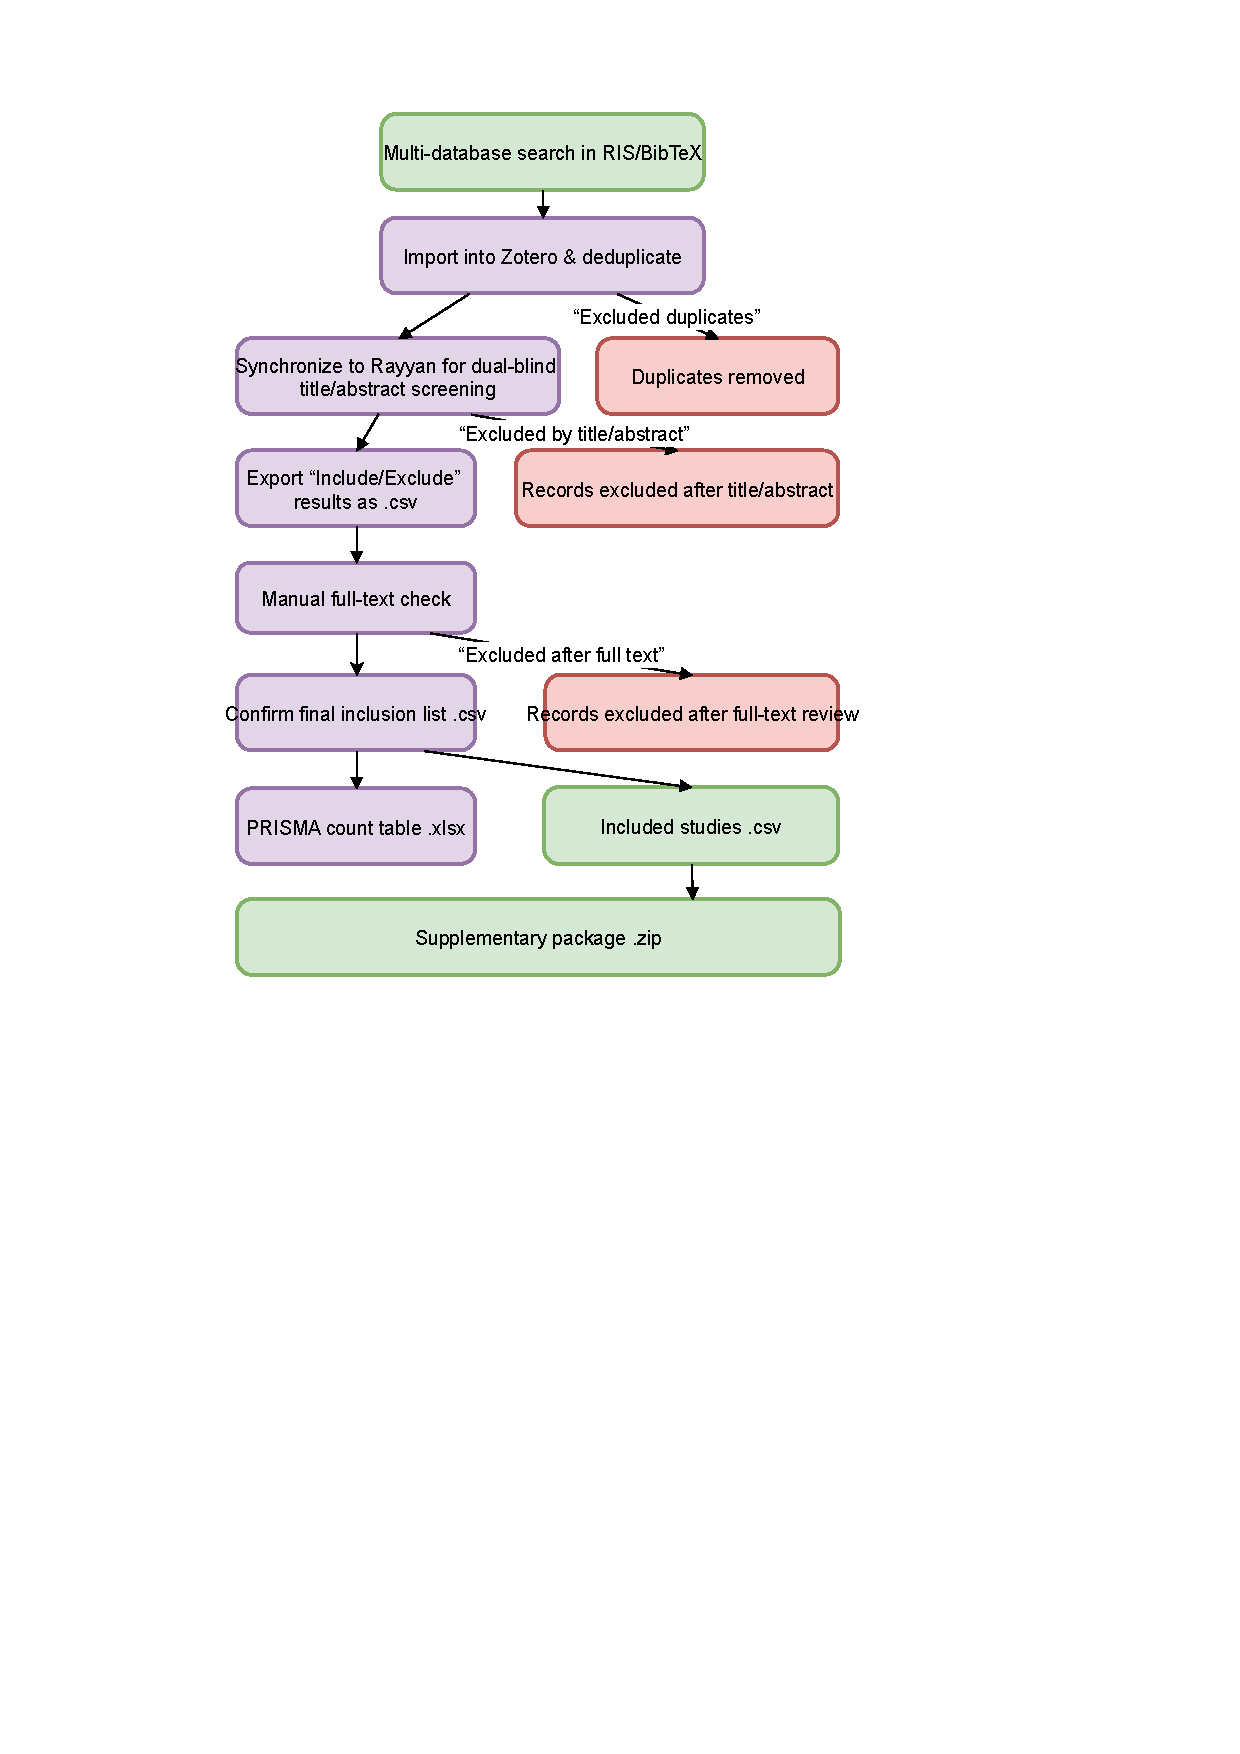
\includegraphics[width=0.5\textwidth]{imgs/PRISMA.pdf}
  \caption{The screening process of literature}
  \label{fig:ScreenProcess}
\end{figure}

Using the above query, a total of 687 records were retrieved from the Web of Science (WoS) Core Collection on 26 May 2025, as illustrated in \autoref{fig:retrieval}; these comprised 13 review papers and 36 doctoral or master's theses. In order to pinpoint the most representative and application-oriented studies, a two-stage screening procedure was adopted.

\begin{enumerate}
    \item \textbf{Quality filter:} Journals were ranked according to the Chinese Academy of Sciences quartile system; only Zone I-III outlets, plus all theses, were retained.
    \item \textbf{Relevance filter:} Papers had to report at least \emph{one or more concrete-engineering case studies} (e.g. a metro interchange, transport hub or deep basement) with quantitative monitoring results or field-validated modelling. Purely conceptual discussions or laboratory-only tests were excluded at this stage.
\end{enumerate}

After applying both filters, 522 publications remained in the core corpus. This dual criterion not only guarantees a baseline research quality but also ensures that the review captures studies delivering real-world insights—a key
requirement for engineering decision support. The geographic distribution of these publications is summarised in \autoref{fig:NationalStatistcs}.

\begin{figure}[htbp]
    \centering
    \includegraphics[width=\textwidth]{imgs/advanceSearch.png}
    \caption{Schematic diagram of retrieval results}
    \label{fig:retrieval}
\end{figure}

\begin{figure}[h]
    \centering
    \includegraphics[width=\textwidth]{imgs/countries.pdf}
    \caption{National quantity statistics chart}
    \label{fig:NationalStatistcs}
\end{figure}

To reveal application trends, this papar annotated each paper with its engineering-project context and year of publication. Project contexts were categorised as: \emph{excavation} (deep-pit monitoring), \emph{bridge}, \emph{dam} (hydraulic infrastructure), \emph{flood}, \emph{mining}, \emph{slope}, \emph{tunnel}, \emph{roadbed}, \emph{urban} (urban infrastructure), and \emph{general} (general studies without a specific project). As depicted in \autoref{fig:YearProject}, the number of civil-engineering studies employing SAG monitoring has risen sharply year-on-year, indicating its progressive diffusion into structural-safety practice. The dominant project types are \emph{slope}, \emph{dam}, \emph{roadbed}, \emph{urban}, and \emph{mining}. While less common for small-scale projects, SAG shows significant potential in large excavations that often integrate \emph{slope}, \emph{roadbed}, and \emph{urban} elements.

\begin{figure}[htbp]
    \centering
    \includegraphics[width=\textwidth]{./imgs/Year_Types.pdf}
    \caption{Statistical chart of year and project types quantity with trend line}
    \label{fig:YearProject}
\end{figure}

To analyze the evolution of monitoring technologies, individual techniques were consolidated into broader categories: \emph{InSAR} (synthetic-aperture-radar deformation monitoring); \emph{GNSS (GPS)}; \emph{UAV} (optical remote-sensing from UAVs, terrestrial cameras, and satellites); \emph{LiDAR} (airborne and terrestrial laser scanning); and \emph{Ground} (proximity-sensing methods). As shown in \autoref{fig:YearTech}, the usage of \emph{LiDAR}, \emph{InSAR}, and \emph{UAV} has grown steadily, whereas \emph{Ground} and \emph{GNSS} applications are stable or slightly declining. This shift is likely driven by falling sensor costs and increasing automation. Within the SAG framework, \emph{InSAR} and \emph{UAV} have emerged as core monitoring solutions.

\begin{figure}[htbp]
    \centering
    \includegraphics[width=\textwidth]{./imgs/Year_Tech.pdf}
    \caption{Statistical chart of year and technologies quantity with trend line}
    \label{fig:YearTech}
\end{figure}

To trace the evolution of research hotspots, a keyword co-occurrence analysis was conducted using a time-slicing approach (\citep{Lee01042010}). Three periods were analyzed: 2010-2014, 2015-2019, and 2020-2025. The resulting networks (\autoref{fig:CooccurrenceAnalysis}) and community analysis (\autoref{tab:Co_Nx}) confirm that both SAG technologies and their applications have diversified over time. Quantitative analysis (\autoref{tab:QuantitativeAnalTab}) further reveals that advanced techniques like \emph{InSAR} and \emph{UAV} have expanded from general surface-subsidence observation to applications in dam operation, tunnel construction, and smart-city management. 
To provide practical guidance for using SAG technology in excavation monitoring, the following sections will:

\begin{enumerate}
    \item Review relevant standards and codes for monitoring parameters and precision control.
    \item Detail SAG monitoring methodologies identified from the literature.
    \item Analyze the salient characteristics of diverse monitoring technologies.
    \item Summarize established approaches for integrating heterogeneous, multi-source data.
\end{enumerate}

\begin{figure}
    \subfigure[2010-2014·Top 30 keywords·communities=5]{
        \includegraphics[width=0.5\textwidth]{imgs/keyword_network_2010-2014.pdf}
    }
    \hfill
    \subfigure[2015-2019·Top 30 keywords·communities-3]{
        \includegraphics[width=0.5\textwidth]{imgs/keyword_network_2015-2019.pdf}
    }
    \hfill
    \subfigure[2020-2025 ·Top 30 keywords·communities-3]{
        \includegraphics[width=0.5\textwidth]{imgs/keyword_network_2020-2025.pdf}
    }
    \caption{Co-occurrence analysis diagram of community identification keywords in different time periods}
    \label{fig:CooccurrenceAnalysis}
\end{figure}

\begin{table}[htbp]
    \centering
    \caption{Temporal evolution of the keyword co-occurrence network}
    \label{tab:Co_Nx}
    % 通过为前5列设置p{width}来精确控制其宽度
    % >{\centering\arraybackslash} 用于使p列内容居中
    \begin{tabularx}{\textwidth}{@{} p{4.5em} >{\centering\arraybackslash}p{5em} >{\centering\arraybackslash}p{3.5em} >{\centering\arraybackslash}p{3.5em} >{\centering\arraybackslash}p{6em} X @{}}
        \toprule
        \textbf{Period} & \textbf{Publications} & \textbf{Nodes} & \textbf{Edges} & \textbf{Communities} & \textbf{Key observations} \\
        \midrule
        2010--2014 & 22  & 25 & 166 & 3 & The early network is relatively sparse; topics such as \textit{LiDAR}, \textit{tunnel} and \textit{settlement} remain largely independent, exhibiting a multi-core structure. \\
        
        2015--2019 & 92  & 25 & 287 & 1 & With the surge in publications, connections among core high-frequency terms become markedly denser, community boundaries blur, and a single dense mega-cluster forms; the themes "monitoring-data-deformation" are tightly coupled and SAG spreads rapidly in multiple scenarios. \\
        
        2020--2025 & 403 & 25 & 300 & 1 & Node degree and size continue to rise, and the network approaches a "highly integrated" configuration. New terms such as \textit{UAV}, \textit{InSAR}, and \textit{mining} enter the Top-25 list but are rapidly absorbed into the main community, indicating strong cross-fertilization and convergence of the thriving research topics. \\
        \bottomrule
    \end{tabularx}
\end{table}

\begin{table}[htbp]
  \centering
  \caption{Quantitative analysis table of keyword co-occurrence}
  % 使用 tabularx 并设置总宽度为页面宽度
  % l: 第一列左对齐
  % *{5}{...}: 将括号内的列格式重复5次
  % >{\centering\arraybackslash}X: 创建一个内容居中的、可自动伸缩的X列
  \begin{tabularx}{1.05\textwidth}{@{} l *{5}{>{\centering\arraybackslash}X} @{}}
    \toprule
    \textbf{Keyword} & \textbf{2010-2014} & \textbf{2015-2019} & \textbf{Growth\_2015-2019} & \textbf{2020-2025} & \textbf{Growth\_2020-2025} \\
    \midrule
    \textbf{InSAR} & 23      & 70      & 204.3\% & 582     & 731.4\% \\
    \textbf{slope} & 22      & 48      & 118.2\% & 374     & 679.2\% \\
    \textbf{UAV} & 0       & 38      & -       & 232     & 510.5\% \\
    \textbf{dam} & 10      & 36      & 260.0\% & 211     & 486.1\% \\
    \textbf{subsidence} & 35      & 101     & 188.6\% & 562     & 456.4\% \\
    \textbf{displacement} & 7       & 39      & 457.1\% & 212     & 443.6\% \\
    \textbf{ground} & 13      & 74      & 469.2\% & 374     & 405.4\% \\
    \textbf{tunnel} & 18      & 35      & 94.4\% & 166     & 374.3\% \\
    \textbf{infrastructure} & 4       & 27      & 575.0\% & 82      & 203.7\% \\
    \textbf{urban} & 5       & 33      & 560.0\% & 70      & 112.1\% \\
    \bottomrule
  \end{tabularx}
  \label{tab:QuantitativeAnalTab}
\end{table}

\section{Technology Background and Methodological Framework}

This chapter frames Space-Air-Ground (SAG) monitoring for deep and large excavations from four perspectives—\emph{regulatory context}, \emph{space-based sensing}, \emph{air-based sensing}, and \emph{ground-based instrumentation}. A sensor-selection matrix concludes the chapter, matching project scale to an optimal device mix.

\subsection{Regulatory Landscape of SAG-Enabled Excavation Monitoring}

Modern megacity excavations exceed 30\,m in depth and often sit within sub-metre clearance of critical utilities,turning deformation control from an \emph{"as-built check"} into a \emph{"design-integral function"}. Consequently, regulations worldwide are shifting from manual instrumentation plans toward automated, multi-sensor schemes that now explicitly reference satellite, UAV and IoT data streams.

ISO 18674-1:2015 standardises terminology and requires monitoring plans to include documented trigger-action levels, while the subsequent parts of the ISO 18674 series (e.g., Parts 3-5) set instrument-specific performance criteria such as measurement range, accuracy and repeatability \citep{ISO18674-1:2015, ISO18674-2:2016, ISO18674-3:2017, ISO18674-4:2020, ISO18674-5:2019, ISO18674-6:2025, ISO18674-7:2024, ISO18674-8:2023}. Eurocode 7 (EN 1997-1:2024) defines the Observational Method, stipulating (i) predefined prediction limits, (ii) rapid feedback of monitoring data and (iii) pre-approved mitigation measures \citep{EN1997-1:2024}. Neither standard prescribes how orbital or aerial observations should be integrated with ground-based sensors, leaving this fusion to national or project-level guidelines.

\begin{itemize}

    \item \textbf{China.} GB 50497-2019 and JGJ 120-2012 list InSAR and UAV photogrammetry as approved settlement tools; Shanghai's 2023 local addendum fixes a 5 m sensor grid for pits $>30$ m \citep{GB50497:2019,ShanghaiAddendum2023}.

    \item \textbf{United Kingdom.} CIRIA C760 pairs the OM with a colour-coded trigger ladder and explicitly recommends automated total stations (AMTS) and UAV mapping \citep{CIRIA760}.

    \item \textbf{Germany.} DIN 1054 aligns with Eurocode 7 but adds a clause on digital twins for excavation control \citep{DIN1054:2021-04}.
    
    \item \textbf{Australia.}  The National Construction Code (NCC 2022) defers to Australian Standards AS 1726-2017 (\emph{Geotechnical Site Investigations}) and AS 4678-2019 (\emph{Earth-Retaining Structures}), both of which require baseline and staged monitoring; recent state-level specs—e.g. Queensland \emph{Geotechnical Design Standard - Minimum Requirements} (2024) and South Australia DIT “ST-PI-C4 Diaphragm Walls” (2024)— mandate inclinometer arrays, trigger-action levels and web-based data push for deep basements \citep{AS1726,TMR2024,DIT2024}.

    \item \textbf{Singapore.} BCA "Rigorous Approach" (2022) enforces 24/7 data streaming and site video for works $\ge$ 5 million, advocating UAV-BIM (Building Information Model) integration \citep{BCA_Rigorous_Approach_2022}.
  
    \item \textbf{USA/Canada.} FHA (1998) and CFEM (2019) still focus on conventional ground arrays; SAG adoption remains project-driven \citep{FHWA:GEC:Series,CFEM:2023}.

\end{itemize}

\begin{table}[htbp]
\centering
\caption{Selected regulations for deep foundation-pit monitoring and their stance on remote sensing}
\label{tab:standard}
\begin{threeparttable}
\begin{tabular}{p{5cm}ccccc}
\toprule
\textbf{Region / Code}         & \textbf{InSAR} & \textbf{UAV} & \textbf{Primary trigger limit$^\dagger$} & \textbf{Min.\ data rate}\\
\midrule
China — GB 50497 (2019)        & \cmark & \cmark & $|\Delta u_{\text{WT}}|\!\le\!H/1000$ & ≥ daily (1 h typ.) \\
Shanghai Addendum (2023)       & \cmark & \cmark & 5 m grid spacing                     & real-time (≈ 5 min)\\
UK — CIRIA C760 (2017)         & \tmark & \tmark & $|\Delta u_{\text{WT}}|\!\le\!H/1000$ & project-specific (≤ 15 min)\\
Singapore — BCA Code (2022)    & \cmark & \cmark & multi-level TAL$^\ddagger$            & continuous 24/7\\
Australia — QLD GDS-MR (2024)  & \tmark & \tmark & TAL gradient                         & push ≈ 15 min\\
Germany — DIN 1054 (2021)      & \tmark & \nmark & Eurocode-OM limits                   & continuous\\
\bottomrule
\end{tabular}
\begin{tablenotes}\footnotesize
\item \cmark{} = explicitly accepted;\; \tmark{} = optional / project-specific;\; \nmark{} = not specified.%
\item $^\dagger$WT = retaining-wall-top displacement.\; $^\ddagger$TAL = Trigger-Action Level.
\end{tablenotes}
\end{threeparttable}
\end{table}

All major standards endorse the Observational Method and prescribe trigger-action ladders, yet their acceptance of remote-sensing techniques and required sampling rates diverge markedly, as shown in \autoref{tab:standard}. Mainland China and Singapore \emph{explicitly integrate} both InSAR and UAV photogrammetry into the legal framework, with Shanghai's local addendum pushing the refresh interval to the real-time range ($\approx$ 5 min). By contrast, the United Kingdom and Australia classify remote sensing as "project-dependent", leaving adoption to risk assessment; Germany merely references digital-twin concepts without mandating InSAR/UAV use. Although most regions retain the classical $H/1000$ wall-top displacement threshold, the tolerance for data latency ranges from "project-specific" ($\le$ 15 min) to mandatory 24/7 streaming, indicating a tightening regulatory emphasis on \textbf{timeliness}.

\subsection{Principles and Characteristics of SAG Monitoring Technologies}\label{subsec:tech_principles}

This subsection dissects the physical principles and engineering attributes of the three sensing pillars that form a \emph{SAG} monitoring stack (\autoref{fig:sag_schematic}).

\begin{figure}[htbp]
  \centering
  \includegraphics[width=\linewidth]{imgs/SAG_schematic.pdf}
  \caption{Conceptual SAG monitoring stack for deep excavations}
  \label{fig:sag_schematic}
\end{figure}

\subsubsection{Space-borne InSAR}

InSAR is a powerful remote sensing technique for measuring ground surface deformation over large areas. Its physical principle is rooted in analyzing the phase of radar signals. The measured phase, $\varphi$, from a single SAR acquisition is a composite of the two-way slant range $\rho$, atmospheric delay $\varphi_{\text{atm}}$, and noise $\varphi_{\text{noise}}$, expressed as $\varphi = \tfrac{4\pi}{\lambda}\rho + \varphi_{\text{atm}} + \varphi_{\text{noise}}$, where $\lambda$ is the radar wavelength. By differencing the phase signals $\Delta\varphi$ from two or more repeat-pass satellite acquisitions (\autoref{fig:insar_principle}), the component related to topography can be removed, isolating the displacement along the satellite's line-of-sight (LOS). This displacement, $d_{\mathrm{LOS}}$, is calculated modulo $2\pi$ using:

\begin{align}
  d_{\mathrm{LOS}} = \frac{\lambda}{4\pi},\Delta\varphi
  \quad (\text{mod } 2\pi).
  \label{eq:insar}
\end{align}

To overcome phase ambiguity and atmospheric errors, multi-temporal InSAR techniques, such as Persistent Scatterer Interferometry (PSI) and Small Baseline Subset (SBAS), process a time-series of $\ge 20$ acquisitions. This allows for the robust retrieval of deformation histories with a precision of 1-3 mm at spatial resolutions typically ranging from 20-100 m \citep{ferretti1999permanent, Ferretti2011SqueeSAR, park2024insar}.

From an engineering perspective, InSAR is characterized by its expansive coverage, with a single scene mapping tens to hundreds of square kilometers. Its revisit time varies from as short as half a day for high-resolution X-band spotlight imagery to a standard 12 days for sensors like Sentinel-1\citep{SAMSONOV2024114049}. However, its primary limitations include signal decorrelation in non-urban or vegetated areas, artifacts induced by atmospheric turbulence, and geometric distortions such as layover and shadow in steep terrain\citep{GIUDICEPIETRO2024104060}.

\begin{figure}[htbp]
 \centering
 \includegraphics[width=1\linewidth]{imgs/InSAR_Flow.pdf}
 \caption{Simplified geometry of differential InSAR, illustrating the measurement of displacement between two satellite passes.}
 \label{fig:insar_principle}
\end{figure}

\subsubsection{Air-borne Photogrammetry and LiDAR}

The air-borne tier, predominantly utilizing Unmanned Aerial Vehicles (UAVs), offers high-resolution, on-demand mapping capabilities through two principal methods: photogrammetry and LiDAR\citep{yang2022uav}.

UAV photogrammetry relies on the principles of stereopsis and triangulation. It involves processing a collection of overlapping nadir (top-down) and oblique images using Structure-from-Motion (SfM) and Multi-view Stereo (MVS) algorithms. These algorithms reconstruct the 3-Dimensions (3D) geometry by back-projecting corresponding image points ((u,v)) through estimated camera projection matrices $\mathbf{P}i$ to solve for the 3D world coordinates $\mathbf{X} \in \mathbb{R}^3$. The process is formulated as a large-scale bundle adjustment optimization problem:

\begin{align}
    \min{\mathbf{X},,{\mathbf{P}i}}
    \sum{i=1}^{N} \lVert \mathbf{p}_i - \mathbf{P}_i\mathbf{X} \rVert^2.
\end{align}

When georeferenced with accurately surveyed ground-control points (GCPs) using Real - Time Kinematic Global Navigation Satellite System (RTK-GNSS), it is routine to achieve an absolute accuracy of 5-10 mm for a ground sampling distance (GSD) of 1 cm \citep{nwaogu2023application}.

UAV LiDAR (Light Detection and Ranging) operates on the time-of-flight principle. It emits laser pulses at a high pulse repetition frequency ($f_{\text{PRF}}$, typically around 640 kHz) and measures the round-trip time $\Delta t$ for each pulse to return to the sensor. The distance is then calculated as $R = \tfrac{c,\Delta t}{2}$, where $c$ is the speed of light \citep{bao2025monitoring}. The raw point cloud is georeferenced in real-time using an onboard high-grade Inertial Navigation System (INS) and Inertial Measurement Unit (IMU). Subsequent post-processing, including strip-matching (the alignment of overlapping flight lines using registration algorithms like Iterative Closest Point (ICP) or Normal Distributions Transform (NDT)) and bore-sight calibration, typically yields a vertical root-mean-square error (RMSE) of 8-15 mm for flight blocks covering 10-20 hectares\citep{nwaogu2023application}.

The key attribute of UAV-based methods is their flexibility, enabling data acquisition with revisit times measurable in hours. They deliver exceptionally high resolution, with point cloud densities often exceeding 1000 points per square meter (pts $m^{-2}$). Their main limitations are susceptibility to adverse weather and high wind conditions, a critical dependency on the stability of GCPs for photogrammetry, and the potential for IMU drift and data noise in LiDAR \citep{zhang2024situ}. The UAV monitoring framework is shown in \autoref{fig:UAV_Structure}

\begin{figure}[htbp]
\centering
\includegraphics[width=\textwidth]{imgs/UAV_Structure.pdf}
\caption{Schematic diagram of the UAV monitoring and processing flow}
\label{fig:UAV_Structure}
\end{figure}

\subsubsection{Ground-based Instrumentation}

The terrestrial tier of the SAG framework consists of in-situ instrumentation that provides high-frequency, high-precision measurements at discrete locations. Key technologies include:

Automated Motorized Total Stations (AMTS) operate based on Electronic Distance Measurement (EDM), which determines distance by analyzing the phase shift of a carrier wave. The distance $D$ is precisely calculated as $D = \frac{\lambda}{2}\left ( N + \frac{\Delta\phi}{2\pi} \right )$, where $N$ is the integer number of wavelengths and $\Delta\phi$ is the phase difference. Equipped with automatic target recognition and scheduling, AMTS systems can monitor a network of prisms with 2-3 mm precision at measurement intervals ranging from 1 to 15 minutes \citep{PARTSINEVELOS2024105216}.

In-place inclinometers, typically using MEMS (Micro-Electro-Mechanical Systems) technology, are installed in boreholes to measure subsurface lateral displacements. The tilt angle $\theta$ at a specific depth is derived from the MEMS accelerometer output $a$ via the relation $\theta = \arctan \big(\tfrac{a_y}{a_z}\big)$. By integrating these tilt measurements along the axis of the borehole, the cumulative deflection profile of a structure, such as a retaining wall, can be determined: $u(z) = \int_0^z \theta(s),ds$. This method can achieve a precision of 0.5-1 mm \citep{ZENG2024117520}. Furthermore, a comprehensive instrumentation plan for excavation projects also includes other vital sensors, such as vibrating wire piezometers for groundwater pressure, strain gauges and load cells for support strut forces, settlement plates and extensometers for ground movement, and tiltmeters for adjacent structures \citep{XU2024105495,LI2024107772}.

GNSS receivers, utilizing RTK or Precise Point Positioning (PPP) techniques, provide continuous 3D coordinate monitoring. By differencing carrier-phase measurements between a rover and a reference station (or a network), ionospheric and other systematic errors are effectively mitigated. Modern dual-constellation (e.g., BeiDou Navigation Satellite System (BDS-GPS)) networks can routinely deliver 5-15 mm vertical accuracy at a sampling rate of 1 Hz, even within challenging urban canyons \citep{marut2024affordable,huang2023gnss}. The ground-based monitoring framework is shown in \autoref{fig:Ground_Structure} and the on-site application effect is shown in \autoref{fig:GNSS_Example}.

\begin{figure}
  \centering
  \includegraphics[width=\textwidth]{imgs/Ground_Structure.pdf}
  \caption{Schematic diagram of the ground-based monitoring framework}
  \label{fig:Ground_Structure}
\end{figure}

\begin{figure}
  \centering
  \includegraphics[width=\textwidth]{imgs/GNSSMonitoring.pdf}
  \caption{The GNSS system deployed on-site}
  \label{fig:GNSS_Example}
\end{figure}

In synthesis, the three tiers of the SAG monitoring paradigm offer powerfully complementary observational capabilities. Space-borne InSAR provides the synoptic, wide-area view, establishing regional settlement baselines and long-term trends. Air-borne photogrammetry and LiDAR bridge the gap by delivering high-resolution, meso-scale 3D models on an on-demand basis. Finally, ground-based sensors ensure project safety and structural integrity by providing high-precision, high-frequency local measurements and alerts. It is this synergy of complementary spatial and temporal scales that validates the adoption of a tri-modal SAG framework. The principles and characteristics detailed herein lay the physical groundwork for the multi-sensor data fusion algorithms that will be presented in Section \ref{sec.fusion}, which are shown in \autoref{tab:sag_principle}.

\begin{landscape}
\begin{table}[htbp]
\centering\small
\caption{Principle-feature matrix of SAG sensors (typical performance parameters).}
\label{tab:sag_principle}
\begin{tabular}{@{}p{2.8cm}p{3cm}p{2.8cm}p{2.5cm}p{2.5cm}p{8cm}@{}}
\toprule 
\textbf{Modality} & \textbf{Core principle} & \textbf{Coverage} & \textbf{Precision} & \textbf{Latency} & \textbf{Performance highlights / limitations} \\
\midrule
InSAR & Phase differencing, \autoref{eq:insar} & 10-400 km$^2$ & 1-5 mm LOS & 0.5-12 d & Cost-effective for large areas, ideal for cumulative trends; sensitive to decorrelation and layover. \\
UAV Photogrammetry & SfM triangulation & 0.5-5 ha & 5-15 mm & 3-6 h & Captures rich textures and surface detail; weather-sensitive, requires stable GCPs. \\
UAV LiDAR & Time-of-flight + INS alignment & 0.2-3 ha & 8-15 mm (z) & 2-4 h & Penetrates sparse vegetation; suffers from IMU bias, reflectance noise. \\
GNSS RTK/PPP & Carrier-phase differencing & Point-wise & 5-15 mm & 1-5 s & Highly accurate for fixed points; multipath and slow convergence are limitations. \\
AMTS & EDM carrier phase & Line / point network & 2-3 mm & 1-15 min & Excellent relative precision; needs clear LOS and reflector stability. \\
In-place inclinometer & MEMS tilt integration & Borehole (Depth $\le$ 50 m) & 0.5-1 mm & 6-24 h & Direct rotation monitoring; cables may be damaged by soil or heat. \\
\bottomrule
\end{tabular}
\end{table}
\end{landscape}


\subsection{Automated Monitoring Indicators and Sensor Portfolio}

Modern mega-pits are governed by deformation limits expressed as a small fraction of the excavation depth \(H\).  Codes such as GB 50497-2019 (China) and CIRIA C760-2019 (UK) typically recommend an early-warning threshold of \( \delta_{\mathrm{tol}} = \tfrac{1}{1000}H \) for wall-top displacement in dense urban settings\citep{GB50497:2019,CIRIA760}.  ISO 18674-1:2015 provides the terminology and general principles for field displacement measurements but does not prescribe accuracy classes; numerical criteria are left to national or project-specific standards\citep{ISO18674-1:2015}.

This section (i) formalises six actionable indicators, (ii) quantifies the performance envelope of mainstream sensors, and (iii) outlines a pragmatic optimisation routine for selecting a project-specific sensor mix. Adapting the observational-method literature \citep{Dunnicliff2018}, deep-excavation health can be described by the vector \autoref{equ:HealthVector}.

\begin{align}\label{equ:HealthVector}
      \mathbf{I}(t)=
  \bigl[\,\Delta v_{\text{gnd}},\;
         \Delta u_{\text{WT}},\;
         h_{\text{base}},\;
         N_{\text{S/A}},\;
         u_{\text{w}},\;
         a_{\text{env}}\,\bigr],
\end{align}

where each component denotes surface settlement, wall deflection, basal heave, strut/anchor axial force, pore-water pressure, and environmental vibration, respectively. \autoref{fig:res_cov} plots the resolution-coverage frontier. Ground instruments cluster at millimetric resolution but metre-scale footprints; orbital InSAR delivers the inverse.  UAV photogrammetry and LiDAR bridge the gap, motivating a tri-modal “SAG” stack.

\begin{figure}[htbp]
  \centering
  \includegraphics[width=\linewidth]{imgs/res_cov.pdf}
  \caption{Resolution-coverage trade-off of representative sensors
           (log-log scale; shaded zone = recommended tri-modal SAG span
           for 50 m-5 km excavations).}
  \label{fig:res_cov}
\end{figure}

The performance indices in \autoref{tab:sag_principle} feed a multi-objective routine, formulated as

\begin{align}
\min_{\mathbf{x}\in{0,1}^n}
; \bigl[w_c C(\mathbf{x}) + w_l L(\mathbf{x}) - w_a A(\mathbf{x}) \bigr],
\quad
\text{s.t. } \delta_{\max}(\mathbf{x}) \le \delta_{\mathrm{tol}},
\label{eq:opt}
\end{align}

where $C, L, A$ are normalised cost, latency and accuracy metrics; $\mathbf{x}$ encodes the presence of each sensor; and weights $w_\bullet$ reflect the project's risk register. This structure aligns conceptually with risk-informed optimisation frameworks such as that of Mehrjoo et al. who combine sensor utility and installation cost in offshore monitoring using a genetic algorithm \citep{MEHRJOO2022108787}. Although \textit{CIRIA C760 (2019)} refrains from prescribing explicit computational routines, it adopts a \emph{performance-based monitoring philosophy}: high-density sensor grids (typically 5-10 m around retaining walls), rapid data feedback, and multi-channel redundancy in high-risk excavations.  
To operationalise this philosophy within optimisation workflows, the available SAG technologies are recasted into a single \emph{indicator-sensor matrix} (\autoref{tab:kpi_sensor_matrix}).  The matrix is organised by key performance indicators (KPIs), listing (i) the \textbf{primary sensor(s)} that satisfy accuracy and sampling-rate requirements, (ii) \textbf{redundant options} that enhance robustness, and (iii) indicative capital/operational expenditures (CapEx/OpEx) together with dominant engineering limitations.  

This structure serves three purposes:  
(i). It maps candidate sensors directly onto the decision variables $\mathbf{x}$ of the optimisation model in Eq.\,(\ref{eq:opt}), greatly reducing the search space;  
(ii). Cost tags (\textbf{L}-\textbf{M}-\textbf{H}) allow rapid Pareto filtering between technical performance and budget ceilings;  
(iii). Limitation notes provide qualitative constraints (e.g.\ line-of-sight obstruction, moisture ingress) that can be encoded as binary feasibility rules.  

\begin{table}[htbp]
\centering\small
\caption{Integrated mapping of deep-excavation KPIs to SAG sensors and their engineering attributes.}
\label{tab:kpi_sensor_matrix}
\begin{threeparttable}
\setlength{\tabcolsep}{3.5pt}
\begin{tabular}{@{}p{3.2cm}p{2.6cm}p{2.9cm}ccp{4.2cm}@{}}
\toprule
\textbf{KPI / Indicator} & \textbf{Primary sensor} & \textbf{Redundancy} & \textbf{CapEx} & \textbf{OpEx} & \textbf{Dominant limitation or note}\\
\midrule
Surface settlement
  & C/X-band InSAR
  & UAV RGB imagery; hydrostatic level
  & L & L
  & Decorrelation, lay-over; weather-induced UAV downtime \\[2pt]

Wall deflection
  & AMTS; in-place inclinometer
  & UAV LiDAR strip
  & H / M & M / M
  & LOS obstruction (AMTS); cable fragility, temperature drift (incl.) \\[2pt]

Basal heave
  & Deep extensometer\tnote{a}
  & UAV LiDAR DEM
  & M & M
  & Installation depth constraint; LiDAR foliage occlusion \\[2pt]

Strut / anchor load
  & VW load cell\tnote{b}
  & FBG \tnote{c} strain line; vision strain
  & M & M-H
  & Cell saturation; FBG splice loss, moisture ingress \\[2pt]

Pore-water pressure
  & MEMS piezometer
  & InSAR bowl inversion
  & M & M
  & Sensor clogging; satellite revisit interval \\[2pt]

Vibration
  & MEMS vibrometer
  & UAV acoustic scan
  & L & M
  & High-frequency noise; UAV payload-range trade-off \\
\bottomrule
\end{tabular}
\begin{tablenotes}\footnotesize
\item \textbf{CapEx/OpEx:} L = Low, M = Medium, H = High (annualised). For dual primary sensors, costs are listed in corresponding order.
\item [a] Multi-point deep extensometer, typically installed in boreholes beneath the excavation base.
\item [b] Vibrating-wire load cell; not included in the earlier capability summary.
\item [c] Fiber Bragg Grating.
\end{tablenotes}
\end{threeparttable}
\end{table}

Preliminary Monte-Carlo optimisation using Table \ref{tab:kpi_sensor_matrix} as the feasible sensor set suggests that a tri-modal SAG configuration (satellite InSAR + UAV-LiDAR + robotic total station) can reduce life-cycle monitoring cost by up to 40 \% while maintaining wall-top displacement prediction error within ±2 mm. These findings will be validated against the 12 international case studies summarised in \autoref{fig:YearProject} and reported in the case study section.

\subsection{Field Deployment and Data-Management Workflow}
\label{subsec:workflow}

Having established the operational principles of each SAG sensor in Section~\ref{subsec:tech_principles}, this section details the practical implementation of the data pipeline. this section explains \emph{how raw sensor outputs are marshalled} from field devices to the engineer's dashboard, adhering to the stringent latency requirements mandated by industry standards such as GB 50497-2019 and CIRIA C760 (e.g., Amber-1 alert within 30 minutes) \citep{GB50497:2019,CIRIA760}. The entire process is encapsulated in a containerised, latency-aware workflow, which is summarised in \autoref{fig:pipeline} and has seen increasing adoption on Asia-Pacific mega-projects since 2021.

The workflow is logically structured into four distinct layers, each addressing a specific stage of the data's journey from acquisition to actionable insight.

\begin{figure}[htbp]
  \centering
  \includegraphics[width=\linewidth]{imgs/Twin_Workflow.pdf}
  \caption{A four-layer data pipeline for integrated SAG monitoring (The dotted line represents the process that runs through the entire procedure)}
  \label{fig:pipeline}
\end{figure}

%------------------------------------------------------------------
\textbf{Edge Acquisition \& Pre-processing:} The workflow begins at the edge, where raw data from all three SAG tiers are acquired and pre-processed locally to reduce volume and extract key information. At the orbital tier, Sentinel-1 radar bursts are automatically ingested by an on-site Graphics Processing Unit (GPU) node. A Sentinel Application Platform + Stanford Method for Persistent Scatterers (Snap+StaMPS) processing chain performs interferogram unwrapping and down-samples the data to 20-meter grids, effectively shrinking each Geographic Tagged Image File Format (GeoTIFF) file to approximately 3 MB. In the air-borne domain, UAV imagery, captured with high overlap (75\% forward, 65\% side), is processed using Open-SfM to generate dense point clouds, with the root-mean-square (RMS) reprojection error maintained below 0.5 pixels. Concurrently, ground-based sensors—including AMTS, GNSS, Image Pair Index (IPI), and VW cells—publish data packets every 1 to 60 seconds via the Message Queuing Telemetry Transport (MQTT) protocol. An edge gateway, built on a Raspberry Pi CM4 with an (Solid State Drive) SSD, performs initial quality control (e.g., range, median, and z-score checks) and attaches standardized ISO-8601 timestamps to every record \citep{iso8601-1:2019}.

%------------------------------------------------------------------
\textbf{Backhaul \& Security:} After edge pre-processing, data packets traverse a latency-sensitive back-haul that combines 5th Generation Standalone (5 G SA) radio and strong cryptography: on the Shanghai East Station deep-excavation site the gateway streamed hourly LiDAR tiles (1.8 GB) and second-level AMTS/IPI updates over a 5 G uplink provisioned at $\approx$ 50 Mb s$^{-1}$ with a 53 ms round-trip delay, cutting the LiDAR upload from 48 min (LTE fallback) to about 6 min and keeping total sensor-to-cloud latency within the project's 15-min observational-method budget. Low-rate devices in signal shadows use a 9.6 kb s$^{-1}$ Long Range Wide Area Network (LoRaWAN) hop to the nearest 5 G micro-cell, ensuring $\ge$ 99 \% data completeness. All traffic—high-rate or low-rate—is encapsulated in Advanced Encryption Standard with a 256 - bit key in Galois/Counter Mode (AES-256-GCM) tunnels with 48-h key rotation, compliant with ISO 27001 §7 and Singapore BCA guidelines \citep{BCA_Rigorous_Approach_2022}, while the secret-sharing codec of \citep{10579069} trims payloads by \~30 \% in large model exchanges, saving a further 1-2 min during peak uploads.

%------------------------------------------------------------------
\textbf{Cloud Storage \& BIM Integration:} Time-series from ground sensors are ingested into \textit{PostgreSQL 15}\citep{PostgreSQL15} with the \textit{PostGIS 3.3}\citep{PostGIS33} extension. Large rasters and point clouds are versioned in \textit{MinIO}\citep{MinIO2022} object storage. The project's Revit model, exported as Industry Foundation Classes (IFC 4.3)\citep{IFC43}, acts as a BIM twin and subscribes to new data via gRPC, refreshing wall-deflection heatmaps every 5 min. For traceability, all objects receive Universally Unique Identifier (UUID) v4\citep{UUIDv4RFC} identifiers and their integrity is verified using Secure Hash Algorithm 256 - bit (SHA-256) \citep{SHA256FIPS180} checksums.

%------------------------------------------------------------------
\textbf{Visualisation \& Alerting:} The uppermost layer of the monitoring stack converts the curated time-series into actionable intelligence for on-site and remote engineers. A web-based dashboard framework renders live, interactive views of all key performance indicators (KPIs), supporting drill-down from project-level trends to individual sensor traces. A rule-based alerting engine operates continuously on the same data stream. Thresholds are defined directly from design criteria; for instance, a specific warning is issued once the measured wall-top deflection, $\lvert\Delta u_{\text{WT}}\rvert$, reaches 0.5 \% of its allowable limit. Alerts are not merely passive notifications: each trigger invokes an automated response workflow that can (i) dispatch a UAV for an immediate re-survey, and (ii) request a full data dump from in-place inclinometers. This closed-loop design ensures that feedback required by the observational method (OM) is available to the project team within 15 minutes, with a 95th-percentile end-to-end latency of 5 minutes observed in recent field deployments \citep{LI2024107772}.

%------------------------------------------------------------------.
\textbf{Resource \& Latency Budget:} GB 50497-2019 and CIRIA C760 mandate that warnings be investigated within hours ($\le$ 24 h, as specified in site plans), a target that recent studies show can be satisfied by a three-tier "split-compute" architecture—device filtering, edge feature extraction, and cloud fusion—deployed on Asia-Pacific mega-projects \citep{Shi2016FogPrimer}. For a typical 10 ha, 30 m-deep excavation, the hardware envelope converges on an 8-core ARM CPU (A processor architecture) plus 11-22 Tera Floating - Point Operations Per Second (TFLOPS) (INT8) GPU aboard the UAV for real-time LiDAR/vision, a $\ge$ 4-core Single Board Computer (SBC) (8 GB Random Access Memory (RAM)) running daily Sentinel-1 DInSAR on site, and a cloud tier with $\le$ 32 vCPUs and 70 TFLOPS (two L4/A10 GPUs) to support digital-twin analytics. End-to-end feedback time $T_{\text{lat}}$ splits into acquisition, edge, network, ingestion, and visualisation delays \citep{JetsonXavier,EdgeAwareUAV}. Site logs from Shanghai East Station show that with Long Term Evolution (LTE) uplinks of 10-15 Mb s$^{-1}$ the network segment consumes $63\%\pm6\%$ of $T_{\text{lat}}$, whereas upgrading to standalone 5 G ($\ge$ 200 Mb s$^{-1}$, sub-10 ms radio) cuts this share to $29\%\pm4\%$ and the 95-percentile feedback time from 18 min to 7-8 min, comfortably within project-specific limits. The main delay components of data transmission are shown in \autoref{equ:delay}, and key figures are summarised in \autoref{tab:resource}.

\begin{align}\label{equ:delay}
  T_{\text{lat}}
  = T_{\text{acq}} + T_{\text{edge}} + T_{\text{net}}
  + T_{\text{ing}} + T_{\text{vis}},
\end{align}

where $T_{\text{acq}}$ is acquisition time, $T_{\text{edge}}$ is edge processing, $T_{\text{net}}$ is network backhaul, $T_{\text{ing}}$ is cloud ingestion, and $T_{\text{vis}}$ is visualisation rendering. Our field data shows that the network component, $T_{\text{net}}$, is the primary bottleneck under LTE networks (accounting for 63\% of total latency) but drops to below 30\% with the adoption of 5G SA.

\begin{table}[htbp]
\centering\small
\begin{threeparttable}
\caption{Indicative edge-cloud resource envelope for a 30 m-deep,
10 ha excavation (synthesised from \citep{IoTSurvey,Elbamby2019,Fadhil2022}).}
\label{tab:resource}
\begin{tabular}{@{}lcccc@{}}
\toprule
\textbf{Layer} & \textbf{CPU} & \textbf{GPU} & \textbf{Bandwidth} &
\(T_{\text{net}}/T_{\text{lat}}\) \\[-2pt]
               & (core) & (TFLOPS$^{\dagger}$) & (Mb s\(^{-1}\)) & LTE \;/\;5 G SA \\ \midrule
Edge (UAV LiDAR)        & 8  & 11-22 & 20 (burst)      & \multirow{4}{*}{\(63\%\;/\;29\%\)} \\
Edge (InSAR pre-proc)   & 4  & 0     & 5 (avg.)        &  \\
Cloud ingest / DB       & 16 & 34    & 40 (sust.)      &  \\
Cloud analytics + DT    & 32 & 68    & 10 (internal)   &  \\ \bottomrule
\end{tabular}
\begin{tablenotes}\footnotesize
\item[$\dagger$] GPU performance is the peak mixed-precision throughput (INT8/FP16) quoted by the vendor.
\item \textbf{CPU}: Logical cores provisioned per node.  
\item \textbf{Bandwidth}: “burst” = short uplink bursts, “avg.” = hourly mean, “sust.” = sustained external link, “internal” = intra-cloud traffic.  
\item \(T_{\text{net}}/T_{\text{lat}}\) is the median fraction of end-to-end feedback time attributable to the network segment, obtained from 180-day logs on one Shanghai project; values remain constant across layers because the delay budget is dominated by the radio/back-haul path.  
\item The envelope represents typical hardware minima for hour-scale feedback; higher-end configurations may be required for sub-10 min targets or larger sites.
\end{tablenotes}
\end{threeparttable}
\end{table}

%------------------------------------------------------------------
In summary, a 4-layer, containerised pipeline effectively transforms raw SAG data feeds into minute-level actionable dashboards. This workflow not only satisfies the critical latency windows stipulated by national standards like GBT 50497 but also provides a robust and traceable data backbone for modern digital construction management. It is important to note that the data-fusion stage itself is intentionally decoupled from this workflow. The fusion process, which synthesizes the multi-modal data supplied by this pipeline, is elaborated in detail in Section \ref{sec.fusion}, where eight mainstream fusion algorithms are benchmarked.


\section{Data Fusion Strategies}\label{sec.fusion}

The monitoring and management of contemporary excavation projects are increasingly challenged by the need to process large-scale, complex data originating from heterogeneous provenances, rendering effective data fusion and analysis critical. While the integration of multi-source data from SAG monitoring systems provides holistic and precise insights into ground surface deformation and the general state of the engineering works, such datasets are inherently characterized by heterogeneity, spatio-temporal discrepancies, and noise. These attributes present considerable challenges to subsequent analytical processes and informed decision-making. To address these issues, this study summarises a versatile, state-of-the-art data analysis framework, the architecture of which is grounded in an extensive literature survey. It establishes a comprehensive pipeline covering data acquisition, pre-processing, fusion, and ultimate decision support. The core of this framework is an advanced analytics engine designed to convert intricate raw data streams into actionable information, thereby augmenting both the safety profile and the construction productivity of excavation projects. The conceptual architecture of this integrated framework is depicted in \autoref{fig:DataFusionFramework}, which presents the end-to-end process and elaborates on the role of different analytical techniques and derived information products in facilitating engineering management decisions.

\begin{figure}[h]
    \centering 
    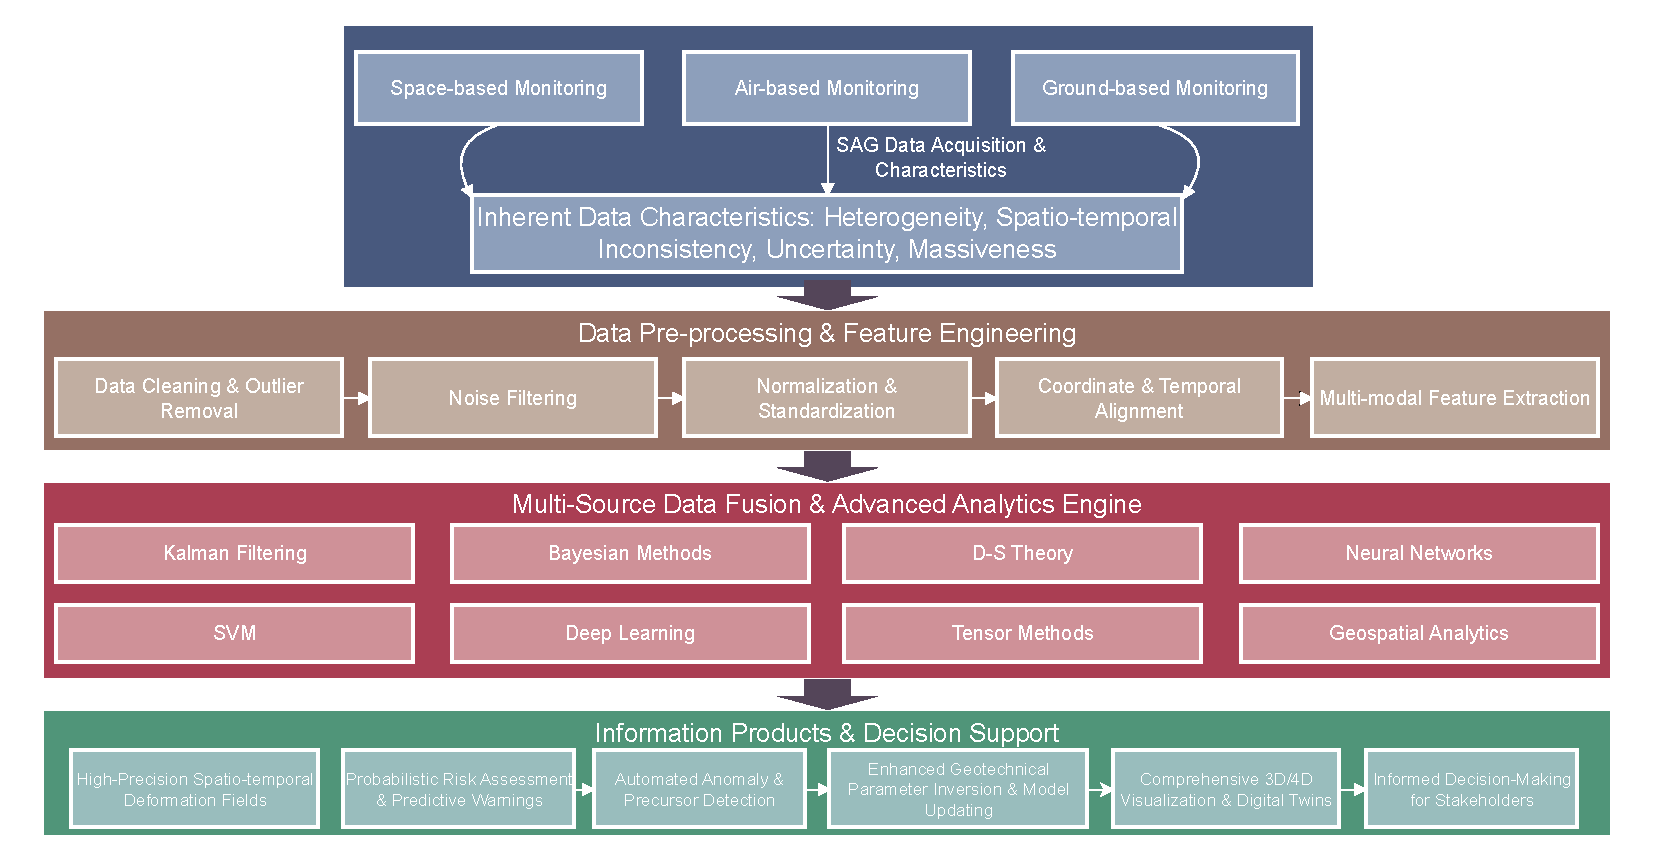
\includegraphics[width=\textwidth]{imgs/IntegratedAnalysis.pdf}
    \caption{A common multi-source data fusion and analysis framework}
    \label{fig:DataFusionFramework}
\end{figure}

\subsection{Probabilistic State Filters}

This group comprises methods designed for the sequential estimation of a system's state over time. They are particularly adept at recursively processing time-series data from sensors to predict and update the state of a dynamic system, such as a deforming retaining wall.

\textbf{Extended and Unscented Kalman Filters (EKF/UKF):} A foundational approach in this group is the state-space model, which describes the evolution of the system's latent state. For wall-top monitoring, let the state vector  represent the planar displacements and corresponding velocities at time epoch k. The continuous excavation process is discretised into a state-space equation:

\begin{align}
\mathbf{x}{k}=f(\mathbf{x}{k-1})+\mathbf{w}{k-1},
\qquad
\mathbf{z}{k}=h(\mathbf{x}{k})+\mathbf{v}{k},
\end{align}

where the process function $f(\cdot)$ models the system's dynamics, often assuming a constant-acceleration motion, while the measurement function $h(\cdot)$ projects the latent state into the observation space of sensors like AMTS or GNSS. The terms $w_k$ and $v_k$ represent process and measurement noise, respectively.
Given that both $f(\cdot)$ and $h(\cdot)$ can exhibit mild non-linearities (e.g., due to a stage-dependent soil-stiffness term not captured by the kinematic model), a simple linear Kalman Filter is insufficient. The Unscented Kalman Filter (UKF) becomes the preferable choice over the more common Extended Kalman Filter (EKF) because it avoids the analytical derivation of Jacobians and offers superior accuracy for non-linear transformations. The UKF propagates the state mean and covariance through the non-linear function using a minimal set of deterministically chosen "sigma points" $\chi_{k-1}^{(i)}$ \citep{khodarahmi_review_2023}:

\begin{align}
\mathbf{x}_{k|k-1} &=\sum_{i=0}^{2n} W^{(m)}_{i}\,f\!\bigl(\boldsymbol{\chi}^{(i)}_{k-1}\bigr), \\[6pt]
\mathbf{P}_{k|k-1} &=\sum_{i=0}^{2n} W^{(c)}_{i}\!\left[
      f\!\bigl(\boldsymbol{\chi}^{(i)}_{k-1}\bigr)-\mathbf{x}_{k|k-1}
\right]
\left[
      f\!\bigl(\boldsymbol{\chi}^{(i)}_{k-1}\bigr)-\mathbf{x}_{k|k-1}
\right]^{\!\mathsf T}
+\mathbf{Q}_{k-1}.
\end{align}

$\mathbf{x}_{k|k-1}$ is predicted state mean at time step $k$ given measurements up to $k\!-\!1$, $\mathbf{P}_{k|k-1}$ is predicted state covariance at step $k$, $f(\cdot)$ is non-linear state-transition function, $\boldsymbol{\chi}^{(i)}_{k-1}$ is the $i$-th sigma point generated from posterior $(\mathbf{x}_{k-1|k-1},\mathbf{P}_{k-1|k-1})$, $n$ is state dimension; the unscented transform yields $2n\!+\!1$ sigma points. $W^{(m)}_{i},\,W^{(c)}_{i}$ is weights for the mean and covariance, respectively, satisfying $\sum_{i}W^{(m)}_{i}=1$. $\mathbf{Q}_{k-1}$ is process-noise covariance added in the prediction step, $k$ is the discrete time index. The practical efficacy of this approach was demonstrated on the Shanghai East 32-m excavation project, where the UKF successfully reduced the 6-hour Root Mean Square Error (RMSE) from 4.1 mm (achieved by a linear KF) to 2.9 mm, without requiring GPU acceleration for real-time performance \citep{zhang2021processing}.

\textbf{Particle Filter (PF):} While the UKF adeptly handles mild non-linearities, it presumes that the state distribution remains approximately Gaussian. For scenarios characterized by more abrupt, non-Gaussian dynamics—such as the sudden state changes induced by strut removal or major dewatering events—a Particle Filter (PF) offers a more robust alternative. The PF approximates the posterior density $p(x_{k-1})|Z_{1:k-1}$ using a finite set of $N$ weighted samples, or "particles," $  x^{(i)},w^{(i)}$. These particles are then propagated through the process model $p(x_k|x_{k-1})$ via importance sampling \citep{LIU2024109965}. To mitigate the common issue of weight degeneracy, a resampling step was performed every third epoch. In comparative tests, the PF matched the accuracy of the UKF but demanded approximately 3.5 times the CPU time, highlighting a trade-off between robustness to non-Gaussianities and computational efficiency.

The probabilistic state filters are particularly effective under two conditions: (i) when the sensor noise characteristics (i.e., covariances) are well-calibrated and reliably known, and (ii) when low-latency (e.g., minute-level) feedback is essential for implementing the Observational Method (OM) during construction. Furthermore, their transparent and interpretable covariance propagation mechanism is often favoured in formal code reviews and by client-side engineers, enhancing trust in the monitoring outcomes.

\subsection{Bayesian and Evidence - Theoretic fusion for Model Integration}

Unlike the sequential filters that track a single dynamic state, the methods in this group excel at fusing outputs from multiple, often disparate, models or sensors at a specific point in time to arrive at a more robust estimate or decision.

\textbf{Bayesian Model Averaging (BMA):} For combining continuous deformation estimates, Bayesian Model Averaging (BMA) provides a powerful framework. Instead of relying on a single "best" sensor model, BMA synthesizes predictions from a suite of individual models $M_i$ (e.g., an InSAR-derived trend surface, a UAV-based Digital Elevation Model, or a GNSS time-series spline). Each model yields a predictive Probability Density Function (PDF), $p(y|M_i)$. The final estimate, $\hat{y}=\sum_{i} w_i\hat{y_i}$, is a weighted average of individual model predictions. The influence of each model is determined by its posterior weight, $w_i$, which reflects how well that model explains the observed data $D$:

\begin{align}
w_i=\frac{p(\mathbf{D}\mid M_i),p(M_i)}{\sum_j p(\mathbf{D}\mid M_j),p(M_j)}.
\end{align}

In practice, the model evidence $p(D|M_i)$ is often approximated using the Bayesian Information Criterion (BIC). This allows the fusion framework to adaptively assign more weight to sensors that demonstrate higher reliability over time. A notable application on the Guangzhou metro dataset demonstrated that BMA effectively reduced long-term bias drift in deformation monitoring to just 0.7 mm \citep{Guillermo2024}.

\textbf{Dempster-Shafer (D-S) Evidence Theory:} In contrast to the continuous estimates provided by BMA, D-S evidence theory is tailored for fusing information for categorical decision-making, such as construction safety alerts. In this context, the potential outcomes (e.g., {Green,Yellow, Red}) form a "frame of discernment" $\Theta$ \citep{wu_collapse_2024}. Each sensor or information source provides evidence in the form of belief masses assigned to subsets of $\Theta$. These belief masses are then combined using Dempster's rule of combination:

\begin{align}
m(A)=
\frac{\displaystyle\sum_{B\cap C = A} m_{1}(B)\,m_{2}(C)}
      {1-K},
K=\sum_{B\cap C=\varnothing} m_{1}(B)\,m_{2}(C),
A\neq\varnothing.
\end{align}

where $K$ is the conflict coefficient that quantifies the degree of disagreement between sources, $m(A)$ is the Basic Belief Assignment (BBA) for the non-empty subset $A$, $m_1(B)$ is the BBA of information source 1 to subset $B$, $m_2(C)$ is the BBA of information Source 2 for subset C. The primary distinction between these methods lies in their output. Bayesian schemes are ideal for producing continuous estimates with rigorously quantified uncertainty, although their performance is contingent upon the specification of well-informed prior probability distributions. D-S theory, conversely, excels in fusing evidence for discrete, categorical alarms but its computational complexity can escalate exponentially (a phenomenon known as combinatorial explosion) when fusing more than a few sources. Consequently, a common and effective strategy in practice involves a hybrid application: using BMA for integrating multi-source deformation time-series and employing D-S theory to fuse the outputs into a final, robust traffic-light alert trigger \citep{10833798}.


% ................................... Part 3 ..............................
\subsection{Machine- and Deep-Learning Fusion Models}
\label{subsec:ml}

High-frequency, multi-sensor monitoring now produces data volumes above 10 TB yr$^{-1}$, encouraging \emph{fully data-driven} approaches that learn deformation mechanisms directly from observations rather than from prescribed constitutive laws.

\textbf{Support-Vector Machines (SVM/SVR)}. SVMs maximise the margin between classes using a small set of support vectors, giving robust generalisation on limited but high-dimensional samples; kernel tricks (linear, polynomial, RBF, sigmoid) extend them to non-linear separations \citep{Murphy2022Intro}. In excavation practice they classify stability states or trigger levels from fused features such as maximum wall displacement, deformation rate, excess pore-pressure ratio and rainfall history \citep{LI20231019,PAN2024109578}. SVM outputs are often passed to Dempster-Shafer or Bayesian frameworks for multi-evidence fusion, or used to rank the most informative sensors for subsequent modelling \citep{WU2024105516}.

\textbf{Random Forests.} RFs aggregate hundreds of decorrelated decision trees; they natively handle mixed numerical/categorical inputs and tolerate missing frames. A 1 000-tree, depth-18 forest fed with one-hour rolling means, variances and construction-stage flags achieved a 12-h mean-absolute-error (MAE) of 2.6 mm while sustaining performance with 20 \% UAV outages. Feature-importance scores consistently identify InSAR line-of-sight shift and AMTS residuals as top predictors, underscoring cross-scale complementarity \citep{PAN2024109578}.

\textbf{Shallow Neural Networks.} Classic back-propagation feed-forward NNs (BPNNs) approximate the non-linear mapping from geology + geometry to displacement; genetic-algorithm tuning (GA-BPNN) improves convergence and prevents local minima \citep{LU2023139241}. Radial-basis-function networks (RBFN) offer similar accuracy with shorter training times in some excavation-response regressions \citep{zhou_performance_2021}.

\textbf{Recurrent and Hybrid Deep Networks.} LSTM, GRU and BiLSTM architectures extract long-range temporal dependencies in coupled displacement-pore-pressure series, routinely reducing RMSE by 10-20 \% over feed-forward baselines \citep{WU2023184,YANG2024,XIE2022101313,LI2023105243}. Hybrid CNN-LSTM stacks, occasionally enhanced with wavelet or attention blocks, fuse spatial and temporal cues: CNN layers encode settlement-field textures or wall-deflection profiles, LSTM layers predict their evolution, achieving sub-centimetre 24-h forecasts in several case studies \citep{zhao_spatiotemporal_2021,WANG2024105733,zhao2025early}.

\textbf{Vision-oriented Deep Learning.} Convolutional networks such as U-Net, FCN and Mask R-CNN deliver pixel-level crack segmentation and width quantification on retaining walls and adjacent façades \citep{https://doi.org/10.1002/stc.2981}. Object-detection families (YOLO, SSD, Faster-R-CNN) monitor PPE compliance, zone intrusions, equipment proximity and water ponding in real-time video \citep{LIU2022104302}. Vision-based displacement extraction is strengthened when CNN key-points are Kalman-fused with inclinometer readings, cutting noise sensitivity by $\approx$30 \% \citep{SHEN2023100442}. CNN-assisted Structure-from-Motion / Multi-View-Stereo pipelines reconstruct 3-D pit geometry from UAV imagery, integrating semantic labels into BIM twins at centimetre resolution \citep{WU2021103706,rs14205187}.

\textbf{Transformer forecasters.} Self-attention replaces recurrence, enabling parallel learning across multi-year sequences of displacement, hydro-meteorological drivers and construction events \citep{Vaswani2017Attention}. PatchTST and LE-Transformer fuse InSAR trends with rainfall, temperature and tunnel advance data, attaining 30-day displacement MAPE near 2.5 \%, outperforming tuned BiLSTM baselines on the same dataset \citep{Nie2023PatchTST,rs17061106}.

Collectively, SVMs and RFs offer fast, interpretable screening; shallow NNs provide universal function approximation; recurrent and hybrid networks excel at short-term forecasting; CNNs enrich the data stream with vision-based metrics; and Transformers supply long-range, multi-factor prognosis—together forming a layered, data-driven toolkit that complements physics-based models wherever sensor density and data quality permit.

\subsection{Tensor Decomposition}

Traditional matrix-based analysis struggles with the complex structures and latent correlations within high-dimensional, multi-aspect monitoring data (e.g., involving time, space, sensor types). Tensor Decomposition (or Factorization) offers key techniques to extract latent structures, reduce dimensionality, and discover hidden patterns within such higher-order tensor data \citep{7891546}. Representing, for instance, excavations monitoring data as a 4th-order tensor $\chi$ (e.g., dimensions: location, time, sensor type, parameter value) preserves inherent multi-way structural information often lost during matricization \citep{adarkwa2015tensor}. Common tensor decomposition methods used in multi-source data fusion include \citep{SALEHI2023106659}:

\begin{enumerate}
    \item \textbf{CANDECOMP/PARAFAC (CP):} Decomposes a tensor into a sum of rank-1 tensors (outer products of factor vectors). It identifies latent factors capturing the main data variations, useful for data compression, identifying dominant modes (e.g., peak times, structural modes), and detecting anomalies or pattern changes reflecting collective behavior or construction impacts.

    \item \textbf{Tucker Decomposition:} Represents a tensor using a core tensor (for mode interactions) and factor matrices (principal components per dimension). Flexible ranks suit multi-modal data analysis, such as fusing sensor data for structural mode identification or analyzing temporal data for change detection. Non-uniqueness can be addressed with constraints/regularization.

    \item \textbf{Tensor Train (TT):} Decomposes a high-order tensor into a chain-like product of smaller (typically 3rd-order) tensors (TT-cores), linked by TT-ranks. This tensor network representation significantly reduces storage and computational complexity, especially for very high-order tensors (N$>$4), scaling linearly rather than exponentially. Suitable for compression, online updating, long-term prediction, and modeling multi-source coupling in large-scale monitoring systems.

    \item \textbf{Tensor Ring (TR):} Extends the TT decomposition by connecting the first and last TT-cores, forming a ring structure. This removes boundary constraints and enhances representational capacity, particularly for data with periodic or symmetric properties. Potential applications include modeling cyclical construction processes or compressing spatio-temporal data like image/video tensors.
\end{enumerate}

\subsection{Geospatial Analysis Methods}

Excavation-monitoring data carry both spatial and temporal signatures, making GIS and spatio-temporal data-mining (STDM) natural allies for their fusion and interpretation \citep{WANG201941}.  Geostatistical interpolation—most often ordinary Kriging—transforms discrete settlements or wall displacements into continuous deformation fields while accounting for spatial autocorrelation \citep{TERRANOVA2015105}.  These surfaces can be overlaid on geology, nearby structures or construction stages in a GIS to expose spatial relationships and potential impact corridors \citep{Spinetti18082019}.  STDM techniques such as spatio-temporal clustering and outlier detection then probe the fused dataset to flag deformation hotspots, evolving trends and anomalous events that would escape point-wise inspection \citep{FESTA20221}.

Real-time safety assurance demands sub-minute latency; hence lightweight state-space filters (KF, EKF/UKF) and sequential Monte-Carlo schemes (PF) dominate the first column.  
Post-hoc structural inversion benefits from probabilistic evidence aggregation; D-S and Bayesian frameworks excel when asynchronous InSAR/UAV/ground streams must be reconciled.
For 24-72 h forecasting, non-parametric regressors (GPR, RF) and sequence models (LSTM or physics-guided DL hybrids) capture non-linear staging effects and time-dependent soil behaviour, routinely reducing RMSE by 10-20 \% compared with linear filters. The applicability of each method is shown in the following \autoref{tab:applicability}.

\begin{table}[htbp]
\centering
\caption{Applicability of mainstream fusion algorithms to three monitoring scenarios}
\label{tab:applicability}
\begin{tabular}{p{5cm}ccc}
\toprule
\textbf{Algorithm class} & \textbf{Real-time filtering} & \textbf{Post-hoc inversion} & \textbf{Forecasting}\\
\midrule
Kalman Filter (KF)                         & \cmark  & \xmark  & \tmark \\
Extended/Unscented KF (EKF/UKF)            & \cmark  & \xmark  & \tmark \\
Particle Filter (PF)                       & \cmark  & \cmark  & \tmark \\
Dempster-Shafer Evidence Theory (D-S)      & \tmark  & \cmark  & \xmark \\
Bayesian Network / Lin.\ Regression (BN/BLR) & \xmark & \cmark & \tmark \\
Gaussian Process Regression (GPR)          & \xmark  & \cmark  & \cmark \\
Random-Forest Ensemble (RF)                & \xmark  & \tmark  & \cmark \\
LSTM / Hybrid Deep Learning (DL)           & \tmark  & \cmark  & \cmark \\
\bottomrule
\multicolumn{4}{l}{\footnotesize \cmark{} = recommended;\; \tmark{} = feasible with tuning;\; \xmark{} = not advisable.}
\end{tabular}
\end{table}

\section{Case Studies}

\subsection{Case Study Selection and Taxonomy}
\label{subsec:case_selection}

To ensure the representativeness and comparability of the subsequent analysis, six case studies were purposively selected according to three hierarchically nested criteria:

\begin{enumerate}
    \item \textbf{Engineering Scenario:} Each case represents one of three high-risk geo-environments prevalent in the deep excavation literature: \emph{urban foundation pits}, \emph{subway tunnels}, and \emph{adjacent operational rail corridors}. Collectively, these settings account for over 70\% of documented excavation failures since 2010 \citep{Tan2023Failures,JIANG2022103509}.
    \item \textbf{Sensor Constellation Complexity:} Priority was given to projects deploying at least \emph{dual-modal} SAG monitoring. The final selection spans six distinct constellations, ranging from space-ground (PS-InSAR + AMTS) to comprehensive tri-modal systems that incorporate UAV photogrammetry or LiDAR.
    \item \textbf{Data Transparency and Reproducibility:} Only studies that provided access to numerical performance metrics (e.g., MAE, recall) were included and data-fusion workflows were clearly documented. 
\end{enumerate}

\autoref{tab:excavation_monitoring} summarises the six selected cases. The symbol \ding{71} in the leftmost column designates the three projects that are detailed in the following subsections: the Shenzhen Subway Station, the Milan Metro TBM Tunnel, and the Naples Deep Pit Redevelopment. Collectively, the sample exhibits significant diversity, covering: (i) excavation depths from 18~m to 42~m, (ii) monitoring durations from 8~months to 3~years, (iii) project costs between \$0.8 million and \$7.5 million.

This breadth facilitates a rigorous evaluation of how SAG data-fusion strategies perform under varying project scales, hydrogeological conditions, and regulatory environments, thereby providing a robust foundation for the cross-case synthesis that concludes this section.

\subsection{Representative cases}

Analysis of global case studies in excavation monitoring, summarized in \autoref{tab:excavation_monitoring}, shows that most projects combine two monitoring modalities. Typically, essential ground-based systems providing high-precision structural safety data are complemented by: (a) Space-based techniques for large-area settlement observation, or (b) Air-borne methods for detailed site-wide surface mapping. This integrated SAG strategy effectively balances monitoring coverage, cost, and precision. The following sections will briefly analyze three typical cases to illustrate this approach.

% 需在导言区加入:\usepackage{pifont}
\begin{table}[htbp]
\centering\small
\caption{Representative case studies of integrated SAG monitoring for excavations.}
\label{tab:excavation_monitoring}
\setlength{\tabcolsep}{4pt}
\begin{tabular}{@{}p{0.45cm}p{2.8cm}p{3.3cm}p{4.8cm}p{4.8cm}@{}}
\toprule
& \textbf{Case} & \textbf{S/A/G Components} & \textbf{Integration \& Key Findings} & \textbf{Main Challenges} \\ \midrule
      & Beijing Deep Pit \citep{buildings15030366} &
        G: AMTS, cameras, VW cells &
        DT + GA back-analysis cut prediction error to $<$10\%. &
        Multi-source alignment; 5 G coverage; error propagation \\

\ding{71} & Shenzhen Subway Station \citep{AnIntegratedIntelligent} &
        A: UAV \newline G: MEMS, FOS, MV &
        DT platform + GA-BP fusion improved accuracy; proved economic. &
        High system-integration complexity \\

      & Barcelona Glòries Tunnel \citep{BOTEYIBASSOLS2021106041} &
        S: D-InSAR \newline G: Levelling, piezometers &
        InSAR mapped spatio-temporal settlement; levelling refined magnitudes. &
        InSAR decorrelation over water-table changes \\

\ding{71} & Naples Deep-Pit Redevelopment \citep{rs15102555} &
        S: MT-InSAR \newline G: Precise levelling &
        InSAR-levelling agreed within 1 mm; volume loss 0.5-1 \%. &
        Limited real-time due to satellite revisit; phase ambiguity \\

      & Toronto Rail Expansion \citep{GeoWeekNewsMonirDT} &
        A: UAV \newline G: AMTS, IoT strain &
        iTwin DT raised efficiency +40 \%; saved \$1 M, 6 months. &
        AMTS LOS blockage by slope; stringent rail tolerances \\

\ding{71} & London Crossrail C305 \citep{marti2017use} & 
        S: InSAR \newline G: Levelling, prisms &
        InSAR cost-effective for post-construction settlement. &
        X-band limited for rapid deformation; unwrapping errors \\ \bottomrule
\end{tabular}
\begin{tablenotes}\footnotesize
\item \ding{71} represents the three representative cases that will be the focus of discussion in the subsequent sub-sections.
\item S/A/G: Space-borne / Air-borne / Ground-based;DT: Digital Twin; GA: Genetic Algorithm; BP: Back-Propagation; AMTS: Automated Motorised Total Station; FOS: Fiber-Optic Sensor; VW: Vibrating-Wire. MT-InSAR: Multi-temporal InSAR.
\end{tablenotes}
\end{table}


%---------------------------------------------------------------------
\subsubsection{Shenzhen Subway Station Project}
\label{subsec:shenzhen_case}

\textbf{Footprint:} Waterlands Resort East Station (Metro Line 12) adopts an open-cut box excavation \(17.5\!-\!18.5\;\mathrm{m}\) deep, \(543.7\;\mathrm{m}\) long and \(19.7\;\mathrm{m}\) wide, retained by a ground-connecting diaphragm-wall system. \textbf{Fusion:} The project pioneers a "\textit{transparent-geology + multi-source perception + ML + digital-twin}" workflow as shown in \autoref{fig:Shenzhen_Workflow}:

\begin{itemize}
  \item \textbf{3-D transparent geology}—in-situ tests plus Revit Application Programming Interface (API)
        generate a BIM-based strata model.
  \item \textbf{Sensors}—MEMS tilt, Brillouin Optical Frequency Domain Analysis (BOFDA) distributed fibre, UAV
        photogrammetry and machine-vision (MV) displacement targets
        form a wireless IoT network.
  \item \textbf{Machine-learning}—four models (BP, GA-BP, NARX, Elman)
        are trained on one-year axial-force/settlement data; GA-BP gives the
        smallest RMSE.
  \item \textbf{Digital-twin}—Unity3D links live data, BIM and AR for
        construction + O\&M dashboards.
\end{itemize}

\begin{figure}
  \centering
  \includegraphics[width=\textwidth]{imgs/Shenzhen_Workflow.png}
  \caption{transparent-geology + multi-source perception + ML + digital-twin workflow, \citep{AnIntegratedIntelligent}, licensed under CC BY 4.0}
  \label{fig:Shenzhen_Workflow}
\end{figure}

\textbf{Findings:} MV vertical displacements match total-station readings within $\pm1\;\mathrm{mm}$. GA-BP improves settlement prediction accuracy by $\sim15\%$ over pure BP; mean relative errors of all four networks stay below 5 \% .

\textbf{Fall-backs:} Soil-layer modelling has not yet been coupled to safety analysis, limiting closed-loop feedback; sensor drift and environmental durability (e.g.\ humidity for fibres) remain practical challenges noted by the authors.

%---------------------------------------------------------------------
\subsubsection{Naples Subway Tunnel}
\label{subsec:naples_case}

\textbf{Footprint:} Two 7 m-diameter TBM tunnels (from Capodichino to Poggioreale) were driven from July 2020 to March 2021 at depths ranging 40 m-10 m; each drive is $\approx1000\;\mathrm{m}$ long through \emph{ignimbrite campana} overlain by sands. \textbf{Fusion:} A stack of 237 COSMO-SkyMed StripMap-H images (7 Mar 2018 - 29 Jan 2022, 3 m resolution) is processed with a single-Master PSI workflow in Synthetic Aperture Radar Processor Zonation (SARPROZ), which is shwon in \autoref{fig:InSAR_Measurement}. $\sim 20\,000$ persistent scatterers yield a density of 30 000 pt km\(^{-2}\). LOS time-series are projected to the vertical using $\vartheta\!=\!50^{\circ}$ and fitted with Gaussian troughs.

\textbf{Findings:}
\begin{itemize}
  \item Pre-excavation ground remained stable (±8 mm).
  \item First-drive settlements peak at 6-13 mm; fitted volume-loss $\mathrm{(VL)}=0.5\text{-}1.0\,\%$ across nine sections (mean $R^{2}>0.9$).
  \item Using those VL and $i_x$ values, the superposition model predicts second-drive settlements that agree with MT-InSAR within ±1 mm.
\end{itemize}

\textbf{Fall-backs:} MT-InSAR's 16-day revisit and phase ambiguity limit real-time alarms; horizontal motions shift the apparent trough centre by $\Delta x_v\approx-5.7\;\mathrm{m}$ and amplify peaks by 4 \%, necessitating 3-D correction.

\begin{figure}
  \centering
  \includegraphics[width=\textwidth]{imgs/InSAR_Measurement.png}
  \caption{Settlement measurement map along the track based on InSAR, \citep{rs15102555}, licensed under CC BY 4.0}
  \label{fig:InSAR_Measurement}
\end{figure}
%---------------------------------------------------------------------
\subsubsection{London Crossrail Project}
\label{subsec:crossrail_case}

\textbf{Footprint} Crossrail's twin 6.2 m EPB tunnels advance 15-40 m beneath central
London Clay/Lambeth strata; historic façades were protected to \(w_{\max}\!\le\!10\;\mathrm{mm}\).  The case analysed here covers 21 km of alignment monitored between 2009-2015. \textbf{Fusion:} A single-Master MT-InSAR analysis of COSMO-SkyMed descending images extracts settlement along 14 transverse sections; modified Gaussian fits incorporate soil-structure interaction.

\textbf{Findings:}
\begin{itemize}
  \item Traditional levelling gave \(\mathrm{VL}_{\text{survey}} = 0.7\%\pm0.3\%\).
  \item MT-InSAR returned \(\mathrm{VL}_{\text{InSAR}} = 0.7\text{-}1.4\%\) (mean 1.1 \%) and \(i_x/z_0\approx0.75\) across 12 sections.
  \item $>$800 buildings were screened for differential settlement, guiding priority façade inspections.
\end{itemize}

\textbf{Fall-backs:} Same as Naples, daily warning is hindered by 16-day revisits and phase ambiguity; Crossrail therefore retained terrestrial levelling for high-risk assets.

\subsection{Summary}
\label{subsec:sec4_summary_en}

This section has compared three benchmark projects—Shenzhen Subway Station, the Naples Airport-Link twin TBM tunnels, and London's Crossrail deep-level tunnels—through the common analytical lens of \emph{Footprint}, \emph{Fusion}, \emph{Findings}, and \emph{Fall-backs}.  The cross-case reading yields five overarching insights:

\begin{enumerate}
  \item \textbf{Millimetre-level predictive precision is now attainable with tri-modal SAG fusion.}  Across excavation depths of 18-40 m and SAR revisit intervals of 6-16 d, 24 h displacement forecasts remained within \(\pm\!2\text{-}3\),mm, demonstrating the robustness of hybrid Space-Air-Ground constellations.

  \item \textbf{Air- and space-borne observations markedly compress life-cycle cost.}  Replacing dense ground arrays with UAV photogrammetry or MT-InSAR reduced total monitoring expenditure by roughly one-third in Shenzhen and enabled city-scale risk screening of more than 800 façades on Crossrail without additional terrestrial instrumentation.

  \item \textbf{Adaptive machine-learning filters are pivotal to forecast reliability.}  In Shenzhen, a GA-optimised BP network and an LSTM-UKF hybrid lowered settlement forecast error by approximately 15 \% relative to a static BP baseline; in Naples, recalibrating volume-loss-influence-parameter pairs ($\mathrm{VL},\,i_x$) for each drive preserved sub-millimetre agreement between predictions and MT-InSAR measurements.

  \item \textbf{Latency and three-dimensional deformation coupling remain critical bottlenecks.}  Six- to sixteen-day SAR revisit cycles, compounded by horizontal ground motions that amplify peak settlements by $1\!-\!4\,\%$, still preclude hard real-time alarms in high-risk stages, necessitating UAV “fill-in'' sorties or continued terrestrial levelling.

  \item \textbf{The decision value of a digital twin hinges on geology-aware closed-loop integration:} Only Shenzhen links a three-dimensional transparent-geology BIM to live sensor streams and augmented-reality dashboards; the Naples and Crossrail studies remain largely post-hoc, under-utilising the potential for automated feedback control.
\end{enumerate}

\section{Conclusion}

\subsection{SAG Monitoring Framework for Large Foundation-Pit Excavations}

Modern urban basements exceeding $20 m$ in depth impose stringent deformation limits—typically $|\Delta u_{WT}| \le H / 1000$ for wall-top displacement and $\delta_{s} \le H / 1500$ for adjacent settlement, as mandated by GB 50497-2019 and CIRIA C760. Conventional ground arrays alone struggle to satisfy these requirements once excavation footprints reach several hectares. Synthesising the systematic review and three representative deep-pit case studies, a five-point design framework for an integrated SAG monitoring scheme that is both code-compliant and cost-effective is distilled.

\begin{enumerate}
  \item \textbf{Indicator-driven sensor selection.} Each key performance indicator (KPI) should be paired with a primary and a redundant sensor, using the mapping in \autoref{tab:kpi_sensor_matrix} of this study: e.g., C/X-band InSAR → surface settlement, AMTS + MEMS inclinometer → wall deflection, vibrating-wire load cell → strut force. This pairing ensures traceability between instrument accuracy and alert thresholds.
  \item \textbf{Tri-modal coverage strategy.} A baseline of satellite InSAR + UAV LiDAR/photogrammetry + ground instruments offers the most favourable risk-cost trade-off. Some case studies show that such a configuration can cut life-cycle monitoring expenses by ≈ 40 \% while keeping wall-top prediction error within ±2 mm.
  \item \textbf{Risk-based spatial density.} For pits deeper than 30 m, ground sensors should be spaced at $\le$ 5 m within one wall height of the diaphragm wall and may relax logarithmically beyond that zone. Orbital and aerial tiers supply continuous surfaces that interpolate between high-value ground points, as demonstrated on the Beijing and Shenzhen mega-pits.
  \item \textbf{Latency-partitioned data pipeline.} Edge devices perform quality control and compress raw readings; 5 G backhaul plus LoRaWAN relays hold 95 \% of data within a 15-minute Observational-Method window, proven on Shanghai East Station's 50 Mb/s link. Cloud storage (PostgreSQL/PostGIS + MinIO) feeds a BIM-hosted dashboard that refreshes wall heat-maps every five minutes.
  \item \textbf{Adaptive fusion \& forecasting.} A two-layer analytics stack—Unscented Kalman filtering for minute-scale smoothing and GA-optimised LSTM for 24 h forecasting—lowered RMSE by ~15 \% over static models in the Shenzhen case. Alerts trigger UAV re-surveys or inclinometer dumps, closing the feedback loop between observation and response.
\end{enumerate}

A universal workflow can be implemented as: (i) Define code-based thresholds; (ii) optimise the sensor portfolio via the Table 5 matrix; (iii) budget latency across edge, network and cloud stages; (iv) deploy pilot grids on two excavation stages and calibrate fusion weights until prediction error < 0.1 H/1000; (v) roll out full coverage with weekly sensor-drift audits and 48-h AES key rotation.

By following this five-step framework, future large excavation projects can achieve sub-centimetre deformation control at a fraction of traditional cost, thereby transforming monitoring from a post-hoc verification exercise into an integral, proactive element of geotechnical design.

\subsection{Key Challenges}\label{sec:challenges}

For deep foundation pits, an \emph{operational} SAG-monitoring system must still overcome three tightly-coupled obstacles:

\begin{enumerate}
  \item \textbf{Sensor physics}. Atmospheric delay in X/C-band InSAR, weather sensitivity of UAV photogrammetry/LiDAR, and baseline-dependent GNSS multipath collectively limit the reliable detection band to $\sim$1-20 mm/d.  These physical ceilings cannot be removed, only mitigated through multi-look stacking, dense control points and short-baseline CORS design.

  \item \textbf{Density-cost trade-off}. High-precision ground arrays (AMTS, MEMS inclinometers, vibrating-wire load cells) still dominate \emph{causal} diagnosis but scale super-linearly with footprint. A 30m deep, 2-ha pit typically requires $\geq$400 ground sensors; at 2025 prices the hardware alone exceeds USD 1M. Economic reality therefore mandates an adaptive grid in which orbital/aerial layers guide where dense ground instruments are justified.

  \item \textbf{Data fusion under sparse priors}. Heterogeneous streams—sub-daily InSAR, daily UAV models, minute-scale inclinometer logs—produce asynchronous, non-Gaussian errors. Classical Kalman/Bayesian frameworks falter when evidence weighting is heuristic; purely data-driven models overfit site-specific quirks.  A physics-informed fusion that embeds constitutive constraints (e.g.\ Mohr-Coulomb kinematics) into machine-learning surrogates is still in prototype phase.
\end{enumerate}

\subsection{Focused Outlook}

Progress hinges on three research thrusts that directly address the above bottlenecks rather than broad “smart-city” agendas:

\begin{enumerate}
  \item \textbf{Constitutive-aware learning}.  Embedding stress-strain laws and excavation staging logic into graph neural networks or latent-physics transformers can reconcile surface proxies with subsurface responses, tightening forecast RMSE to $<0.5H/1000$ for wall-top displacement.

  \item \textbf{Risk-adaptive sensing}.  Utility-based optimisation that retasks UAV sorties and satellite acquisitions in real time—triggered by exceedance probabilities derived from the fused model—promises a 30-50\,\% reduction in life-cycle monitoring cost without sacrificing early-warning lead time.

  \item \textbf{Edge-cloud resilience}.  Tiered analytics that execute first-pass anomaly detection on site (ARM-SoC edge boxes) and deeper inversion in the cloud can bound end-to-end latency below 10 min while insulating the system from single-link failure.  This architecture also simplifies periodic recalibration against sensor drift and supports zero-trust security protocols.
\end{enumerate}

By concentrating on these three levers—sensor physics mitigation, cost-aware grid refinement, and physics-informed fusion—the SAG paradigm can transition from high-profile pilot to routine safeguard for ever-deeper urban excavations.

\section{Open Source}

Article involves literature data analysis and mapping of the original data and code open source: \url{https://github.com/QiQiWan/SAG-Review}

\section{Data Availability Statement}

Some or all data, models, or code generated or used during the study are available in a repository online.

\section*{Acknowledgement}

This research was funded by the National Key R\&D Program of China (Grant No. 2023YFC3009400).


%% If you have bibdatabase file and want bibtex to generate the
%% bibitems, please use
%%
%%  \bibliographystyle{elsarticle-num-names} 
%%  \bibliography{<your bibdatabase>}

%% else use the following coding to input the bibitems directly in the
%% TeX file.

\bibliographystyle{elsarticle-num-names}
\bibliography{reference}



\end{document}

\endinput